\documentclass{article}
\usepackage{float}
\usepackage{textcomp}
\usepackage{graphicx}
\usepackage{booktabs}
\usepackage{color}
\usepackage{verbatim}
\usepackage{listings}
\usepackage{underscore}
%\usepackage{showkeys}
%\usepackage{float} % here for H placement parameter
\usepackage{flafter} 
\setcounter{secnumdepth}{5}
\usepackage[bookmarks=true]{hyperref}
\author{Mirko Mantovani (893784), Matteo Marziali (893904)} 
\date{\today}
\title{Politecnico di Milano
	\\A.A. 2017\@-\@2018
	\\Software Engineering II project \\ \textbf{Travlendar+}
	\\\textbf{R}equirements \textbf{A}nalysis \\and\\ \textbf{S}pecifications \textbf{D}ocument}
	\hypersetup{pdftitle={Software Requirement Specification},    % title
	pdfauthor={Mirko Mantovani, Matteo Marziali},                     % author
	pdfsubject={RASD},                        % subject of the document
	colorlinks=true,       % false: boxed links; true: colored links
	linkcolor=blue,       % color of internal links
	citecolor=blue,       % color of links to bibliography
	filecolor=black,        % color of file links
	urlcolor=purple,        % color of external links
   }
\begin{document}
\maketitle
\begin{center}
	
\includegraphics[width=5cm]{polimi-logo}
\end{center}
\clearpage
{\hypersetup{hidelinks}\tableofcontents}
\clearpage

\section{Introduction}

\subsection{Purpose}
The main purpose of Travlendar+ is to create a software that allows users to easily manage their daily meetings and commitments, by providing some useful features such as finding the best means of transport to reach the appointment place and easily know the quickest route available to be punctual.\\
Specifically, we want to realize a product which is able to:
\begin{itemize}

\item Provide a calendar and the possibility to memorize events and appointments on it.

\item Automatically compute and account for travel time between appointments to make sure that the user is not late for them.

\item Automatically generate warnings to notify the user that at least two meetings are overlapping.

\item Provide routes and travels according to user preferences about the preferred/prohibited travel means and daily breaks set.

\item Provide the possibility to add reminders for a meeting in order to prevent the users forgetting their appointments.

\item Allow the users to modify appointment schedules.

\item Automatically notify people involved in a specific meeting if the user is late and has selected this feature previously. 


\end{itemize}

On the other hand, the purpose of this paper is to define in a detailed way all the functions and requirements of our application.\\ In doing this, we start focusing on a brief overview to characterize the product with relevance to its interaction with the world, then we will proceed deeply in analysing which functions are relevant and should be provided, and which requirements are needed to the stakeholders. 



\newpage
\subsection{Scope}
The main focus of our system design phase will be to create an application capable of reaching the vast majority of users. Thus the architecture must be designed with the intent of being maintainable and extensible, also forseeing future changes.
It should also be flexible enough in order to make future integration of features or adaptations and deploy on other type of platforms and devices as easy as possible. This document aims to drive the implementation phase so that cohesion and decoupling are increased in full measure. In order to do so, individual components must not include too many unrelated functionalities and they should reduce interdependency between one another.

\subsubsection{The world and the machine}
\begin{figure}[htp]
	\begin{flushleft}
		The first model of the system to be presented is the model ``The world and the machine'' by M. Jackson and P. Zave. This model highlights the division between phenomena that happen entirely either in the world or in the machine, and those that are shared between the two of them.
	\end{flushleft}
	\centering
	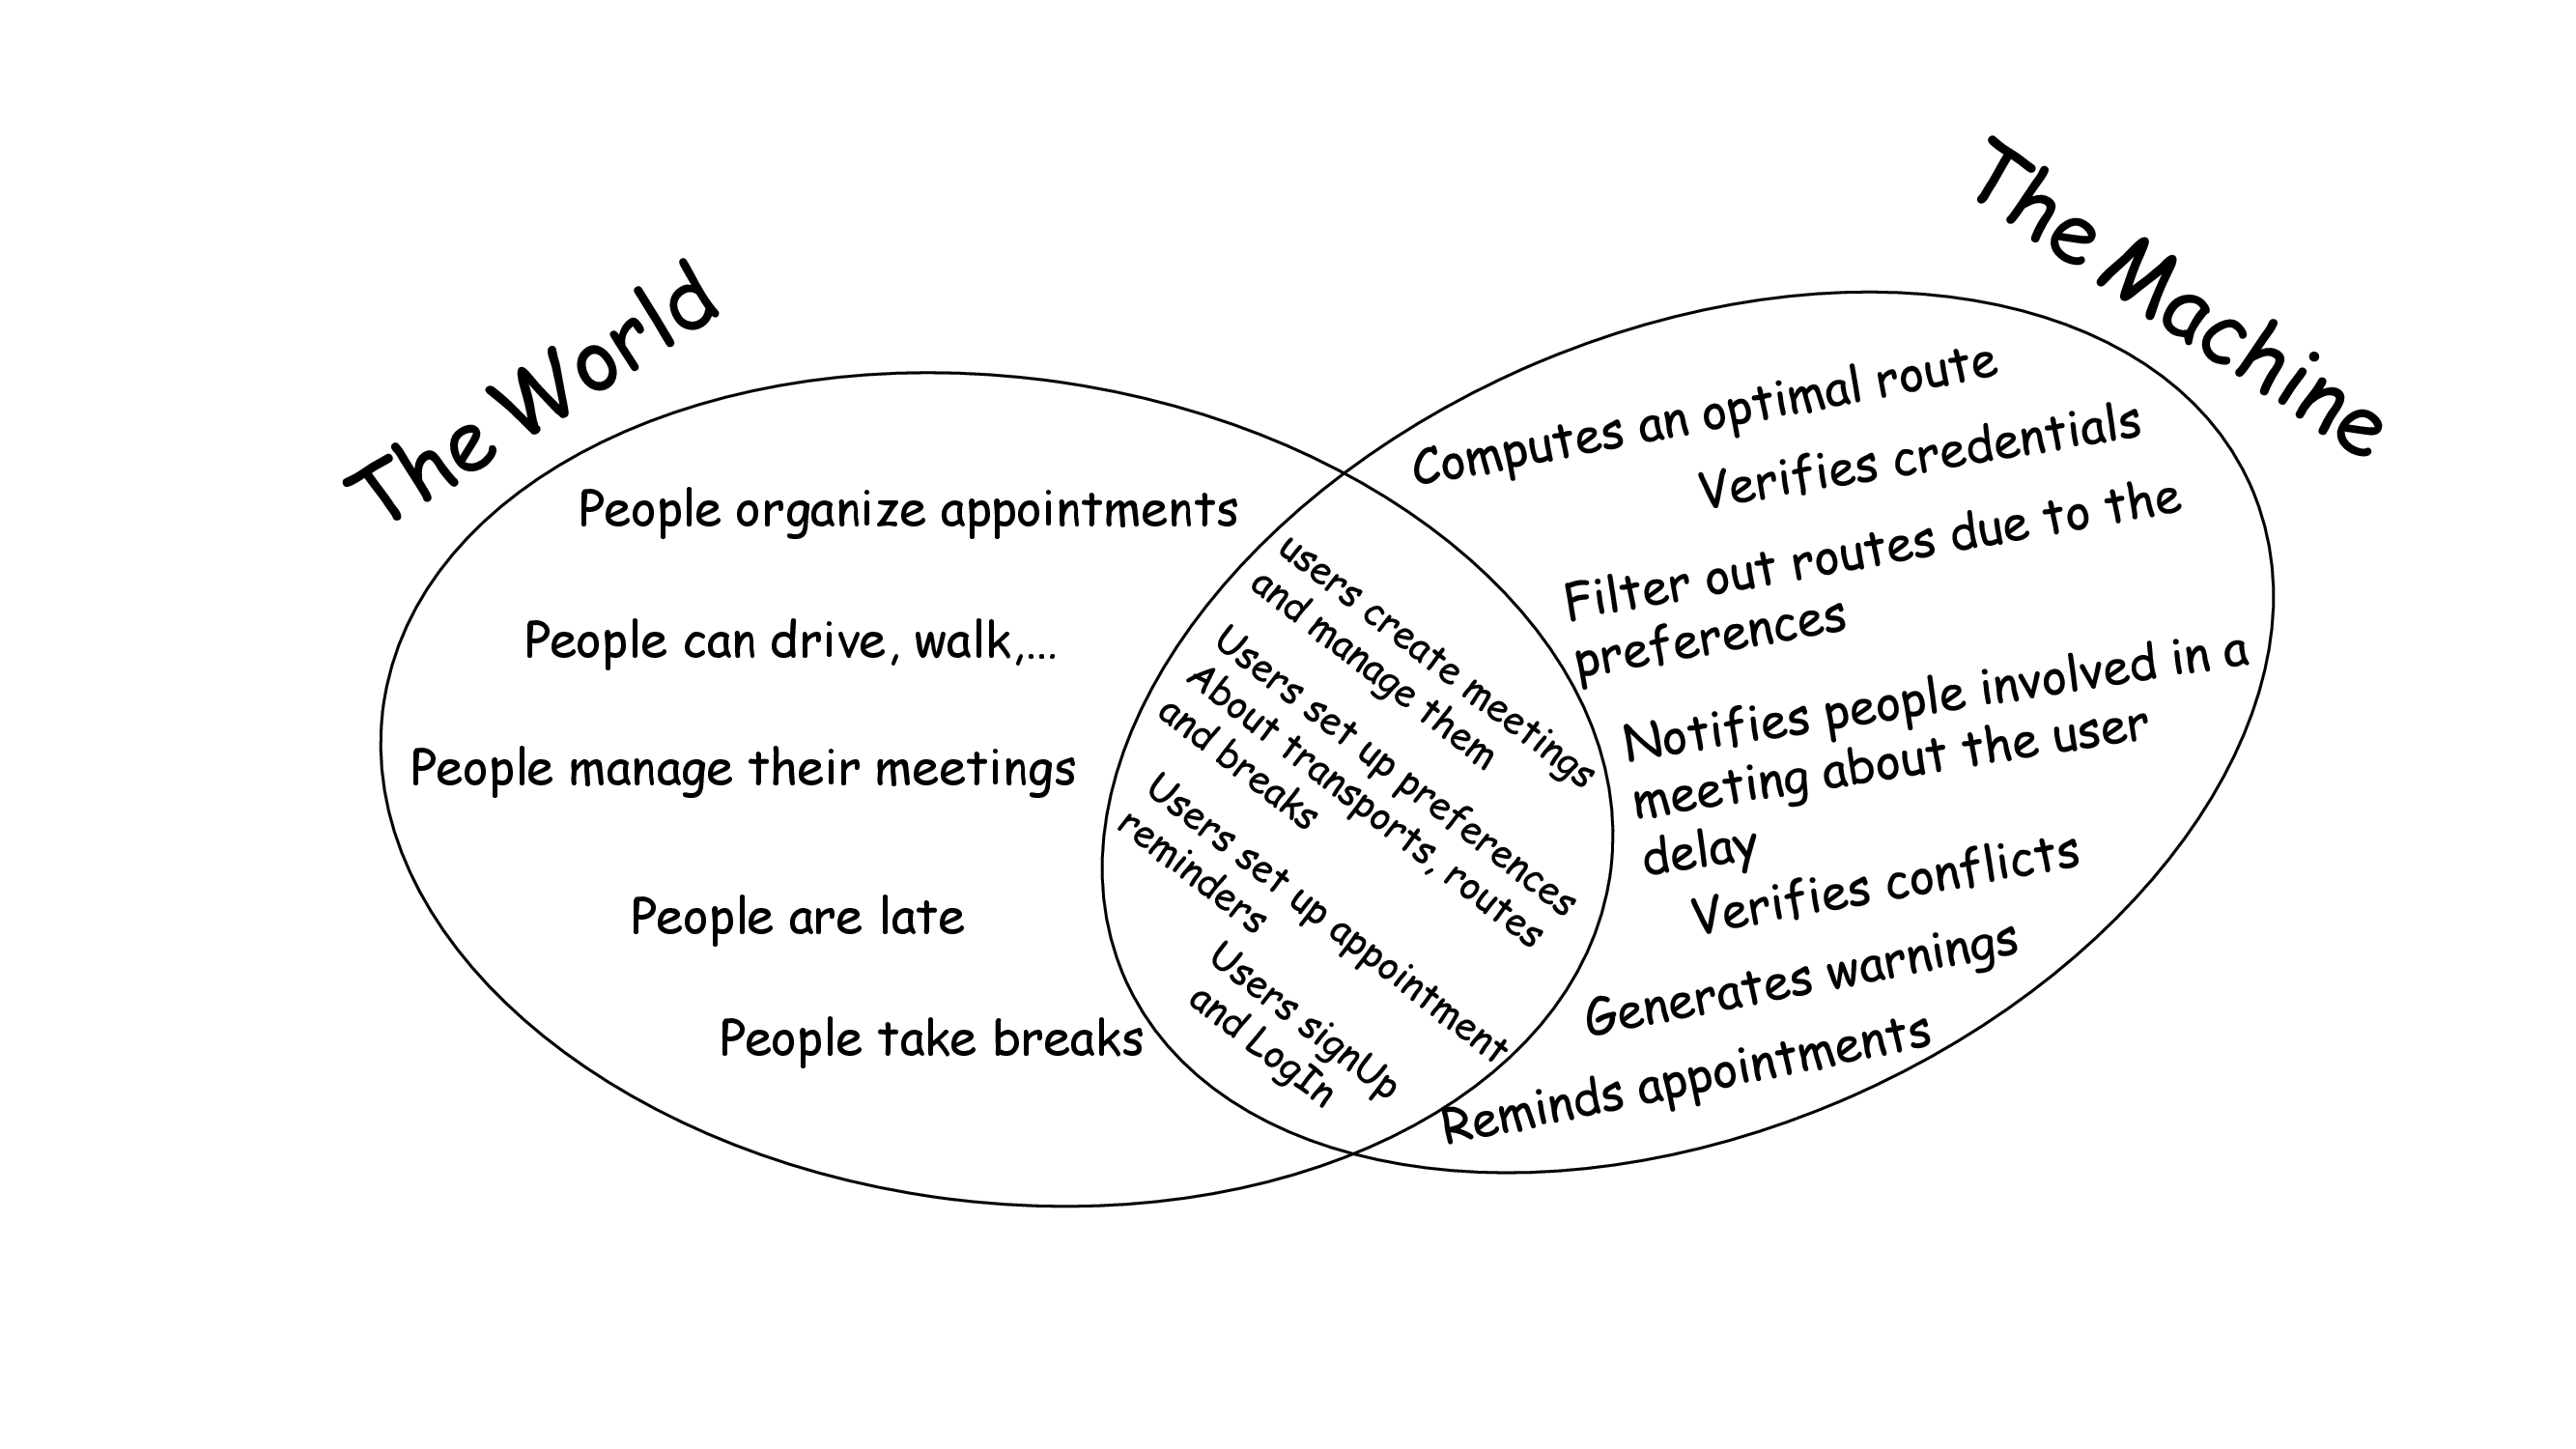
\includegraphics[width=\textwidth]{images/World-Machine}
	\caption{The world-machine chart.}
	\label{fig:world-machine}
\end{figure}

\clearpage
\subsection{Goals}
\begin{itemize}

\item[\hypertarget{G1}{G1}]  Memorizing and organizing both events and appointments on the calendar. 

\item[\hypertarget{G2}{G2}] Being sure to reach the appointment location in time avoiding delays. \label{G2}

\item[\hypertarget{G3}{G3}] Being sure not to schedule overlapping meetings. \label{G3}

\item[\hypertarget{G4}{G4}] Being able to use only travel means that fit with user preferences. \label{G4}

\item[\hypertarget{G5}{G5}] Preventing the user to forget an appointment. \label{G5}

\item[\hypertarget{G6}{G6}] Allowing the users to modify appointment schedules. \label{G6}

\item[\hypertarget{G7}{G7}] Notifying other people involved in a meeting about user eventual delay. \label{G7}

\end{itemize}
In order to clarify and simplify the reading, a traceability table is provided to easily follow the mappings among Travlendar+ goals, functions and constraints: \\
\begin{flushleft}

\begin{table}[htp]

\begin{tabular}{l|l|l|l|l|}
 GoalID&FunctionsID&ConstraintsID&UseCasesID&Other references\\
\hline
\hline
\hyperlink{G1}{G1}&\hyperlink{F2}{F2}&\hyperlink{C4}{C4}, \hyperlink{C5}{C5}, \hyperlink{C6}{C6}, \hyperlink{C7}{C7}&\autoref{tab:meetingcreationtab}&\autoref{fig:meetingcreationprocess}, \autoref{fig:meetingcreation}\\
\hline
\hyperlink{G2}{G2}&\hyperlink{F6}{F6}, \hyperlink{F8}{F8}&\hyperlink{C10}{C10}, \hyperlink{C11}{C11}&-&-\\
\hline
\hyperlink{G3}{G3}&\hyperlink{F4}{F4},&\hyperlink{F9}{F9}&-&\autoref{tab:warningsolving}\\
\hline
\hyperlink{G4}{G4}&\hyperlink{F3}{F3}&\hyperlink{C10}{C10}, \hyperlink{C11}{C11}, \hyperlink{C13}{C13}&\autoref{tab:activatedeactivatemean}, \autoref{fig:specifyuserpreferences}&-\\
\hline
\hyperlink{G5}{G5}&\hyperlink{F7}{F7}&\hyperlink{C12}{C12}&\autoref{tab:reminderaddition}&-\\
\hline
\hyperlink{G6}{G6}&\hyperlink{F8}{F8}&\hyperlink{C4}{C4}, \hyperlink{C5}{C5}, \hyperlink{C6}{C6}, \hyperlink{C7}{C7}&-&\autoref{fig:schedulemanagement}, \autoref{fig:meetingstatemachine}\\
\hline
\hyperlink{G7}{G7}&\hyperlink{F5}{F5}&\hyperlink{C12}{C12}&\autoref{fig:schedulemanagement}&-\\
\hline
-&\hyperlink{F1}{F1}&\hyperlink{C1}{C1}, \hyperlink{C2}{C2}, \hyperlink{C3}{C3}&\autoref{fig:userpage}, \autoref{tab:signup}, \autoref{tab:login}&-\\
\hline

\end{tabular}

\caption{Traceability table } 
\label{tab:traceabilitytable}

\end{table}

\end{flushleft}
\clearpage

\subsection{Definition and Acronyms}

\subsubsection{Definitions}
\begin{itemize}

\item  \textbf{App:} this is the abbreviation for application, in particular this term is used meaning a mobile application.

\item  Delay notification function: this phrase refers to the function which allows to notify the participants of a meeting through an email in case the user is late.

\item  \textbf{Travel:} a travel is any suggested path that goes from the starting point to the meeting location.

\item  \textbf{Route:} this term is used as a synonym of travel.

\item  \textbf{Warning:} warning is the word used to define the conflict between two meetings.

\item \textbf{Meeting conflict:} this means the timings of meetings are incompatible, in other words the user can't reach in time the second meeting if the first meeting finishes on time

\item  \textbf{Calendar:} the calendar contains the list of meetings and is grouped by day.

\item  \textbf{Meeting:} is an important keyword of the application, it includes all the informations of an appointment.

\item  \textbf{Reminder:} a reminder is a sort of an alarm triggered at a certain time before an appointment is starting.


\end{itemize}

\subsubsection{Acronyms}
\begin{itemize}
	\item \textbf{API}:\@ application programming interface; it is a set of routines, protocols, and tools for building software applications on top of this one.
	
\subsection{Revision}
\begin{itemize}
\item \textbf{V2 on \date{\today}:} Complete revision of component diagrams and database after implementation. Added new user interface screens on web application.
\end{itemize}


\subsection{Actors}
\begin{itemize}
	\item \textit{Guest}: This actor plays the role of a person who is not registered and thus logged in. Obviously the signup and the login operations would allow the guest to upgrade his status to 'user'.
	\item \textit{User}: This actor refers to the condition of people already signed up and logged in. 

\end{itemize}

\subsection{References}
\begin{itemize}
	\item The document with the assignment for the project
	\item The IEEE Standard for SRS 
\end{itemize}
\subsection{Document Structure}
This document is structured in three parts:
\begin{itemize}
	\item \textbf{Introduction}: In the first introductory section, we give a short description both of the goals and of the environment which our app has to deal with. Moreover, we explain some notes useful to understand and read the whole paper. 
	\item \textbf{Overall Description}: gives a general description of the application, focusing on the context of the system, going in details about domain assumptions and constraints. The aim of this section is to provide a context to the whole project and show its integration with the real world and showing the possible interactions between the user, the system and the world itself. 
	\item \textbf{Specific Requirements}: this section contains all of the software requirements to a level of detail aimed to be enough to design a system to satisfy said requirements, and testers to test that the system actually satisfies them. It also contains the detailed description of the possible interactions between the system and the world with a simulation and preview of the expected response of the system with given stimulation. 
\\Finally, we express the requirements through the Alloy model, which allows us to define the interactions, the functions and the constraints that characterize Travlendar+ using a formal language.\\
The document ends with a short note about the effort spent in producing it and at last you can also find useful references.
\end{itemize}

\clearpage
\section{Overall description}

\subsection{Product perspective}
Our idea is to create a personal companion application to help users managing and organizing their daily life. According to this intention, we would like to realize an extremely friendly user interface and a lightweight software in order to make Travlendar+ affordable to many people and runnable by many devices.
In order to make use of every functionality the devices require GPS service and an internet connections for most of the services.
Since Travlendar+ is going to offer many routes depending on different travel means, it will necessarily have to interact with many institutions such as public transport and car/bike sharing providers. This aspect will affect both the software and the hardware design. Indeed, it is necessary to query data about the shared cars, bikes and the taxis location around the city and to retrieve information about trains and buses schedules. 
Hence, our system must be very fast and dynamic to support a huge number of query in a few seconds, moreover to interview external databases it's strictly required that the users have an active internet connection. 
Concerning the hardware, we intend to have a database which only contains username and password of all our customers. For sure, it seems useless having a database for those kinds of data but in our idea this choice allows the app to be updated and improved easily in the future, for instance saving on the database clients' routes and meetings. 




\clearpage

\subsection{Product functionalities}

\begin{itemize}

\item \textbf{[\hypertarget{F1}{F1}] Signup and Login}: \\Travlendar+ users must sign up the first time they intend to create a meeting and further usages of the app will require a login to access all its functionalities.
\item \textbf{[\hypertarget{F2}{F2}] Meeting creation}: \\This is the most important function of the app, it allows to generate an event related to an appointment. It requires the user to define all the details such as date, time, location, starting point, preferences etc. 
\item \textbf{[\hypertarget{F3}{F3}] Preferences set up}: \\An important feature of Travlendar+ consists in allowing the user to filter out specific routes depending on some constraints about the travel, or to set break-dedicated time slots.
\item \textbf{[\hypertarget{F1}{F1}] Warnings management}: \\ In case a warning is generated by the system due to a possible overlap among two or more meetings, the user must solve the warning. In other words, the user has to decide wheter he wants to ignore the overlap notification or he intend to modify some meetings to be sure that he can reach and participate to all his appointments.
\item \textbf{[\hypertarget{F4}{F4}] Delays management}:  \\If the app had noticed, according to the estimated travel time, that the user is in late, and he previously had inserted the email address of the meeting’s participants, Travlendar+ would notify them about the delay. 
\item \textbf{[\hypertarget{F5}{F5}] Route generation}:\\ the main hidden function of Travlendar+ is to automatically compute and suggest to the user the best travel among those which fit the preferences he has selected.
\item \textbf{[\hypertarget{F6}{F6}] Reminder management}: The applications allows users to set up reminders for a certain Meeting in order for the user not to be late for it.
\item \textbf{[\hypertarget{F7}{F7}] Recurrent events management}:\\ The smartest function Travlendar+ will offer; it consists in allowing the user to select events to be rescheduled periodically just creating one meeting. Done this choice, the app. Automatically manages to  reschedule the specific meeting according to the period that the user establish, for instance one week, one month.
\item \textbf{[\hypertarget{F8}{F8}] Update meetings}: \\This function is both basic and relevant, it allows the user to customize his meetings after their creation. In other words, through this functionality the user can modify each one meeting details, even in case of a warning is generated.


\end{itemize}

 

In order to clarify and simplify the reading, a traceability table is provided to easily follow the mappings among Travlendar+ goals, functions and constraints: \\
\begin{flushleft}

\begin{table}[htp]

\begin{tabular}{l|l|l|l|l|}
 GoalID&FunctionsID&ConstraintsID&UseCasesID&Other references\\
\hline
\hline
\hyperlink{G1}{G1}&\hyperlink{F2}{F2}&\hyperlink{C4}{C4}, \hyperlink{C5}{C5}, \hyperlink{C6}{C6}, \hyperlink{C7}{C7}&\autoref{tab:meetingcreationtab}&\autoref{fig:meetingcreationprocess}, \autoref{fig:meetingcreation}\\
\hline
\hyperlink{G2}{G2}&\hyperlink{F6}{F6}, \hyperlink{F8}{F8}&\hyperlink{C10}{C10}, \hyperlink{C11}{C11}&-&-\\
\hline
\hyperlink{G3}{G3}&\hyperlink{F4}{F4},&\hyperlink{F9}{F9}&-&\autoref{tab:warningsolving}\\
\hline
\hyperlink{G4}{G4}&\hyperlink{F3}{F3}&\hyperlink{C10}{C10}, \hyperlink{C11}{C11}, \hyperlink{C13}{C13}&\autoref{tab:activatedeactivatemean}, \autoref{fig:specifyuserpreferences}&-\\
\hline
\hyperlink{G5}{G5}&\hyperlink{F7}{F7}&\hyperlink{C12}{C12}&\autoref{tab:reminderaddition}&-\\
\hline
\hyperlink{G6}{G6}&\hyperlink{F8}{F8}&\hyperlink{C4}{C4}, \hyperlink{C5}{C5}, \hyperlink{C6}{C6}, \hyperlink{C7}{C7}&-&\autoref{fig:schedulemanagement}, \autoref{fig:meetingstatemachine}\\
\hline
\hyperlink{G7}{G7}&\hyperlink{F5}{F5}&\hyperlink{C12}{C12}&\autoref{fig:schedulemanagement}&-\\
\hline
-&\hyperlink{F1}{F1}&\hyperlink{C1}{C1}, \hyperlink{C2}{C2}, \hyperlink{C3}{C3}&\autoref{fig:userpage}, \autoref{tab:signup}, \autoref{tab:login}&-\\
\hline

\end{tabular}

\caption{Traceability table } 
\label{tab:traceabilitytable}

\end{table}

\end{flushleft}
\clearpage

\subsection{User characteristics}
According to our idea, Travlendar+ does not have a specific customers range, it is supposed to be used by both male and female, whatever their age is.
Obviously, considering that we intend to produce a mobile application, people who want to use Travlendar+ should be familiar with a portable device like a smartphone or a tablet. 
For sure, users should respect several requirements due to the travel means they are going to take. For instance, when cars are selected as active in the means of transport list, the user is supposed to have a valid driver licence, taking the bus is allowed only with an appropriate ticket.
Moreover, users interested in dealing with Travlendar+ services must have an e-mail address, primarily due to register and authenticate themselves, secondly to use the delay notification function.



\subsection{Assumptions and dependencies}

\subsubsection{Domain Assumptions}
\begin{itemize}
\item The user is supposed to attend every meeting

\item A meeting should not take more time than expected.

\item If a user has a meeting in a specific location, he's supposed to be there at the end of the meeting, and the app will compute a route based on that information

\item The Metros and buses are supposed to be on time, travel times are calculated based on the expected route duration.
\end{itemize}

\subsubsection{General Assumptions}

\begin{itemize}

\item[A1] Signup and Login

Considering that the assignments provided do not say much generally about users without any reference to a possible signup or login, we assume that the registration is mandatory to create the first meeting, then every access to the app requires the login to manage each event saved. Please note that login parameters could be memorized to save and recover easily a user instance.

\item[A2] Meeting management

According to the requirements, we want to develop a system which allows the user to set his preferences with regards to the travels. Moreover, we decide that he can also cancel or anticipate/postpose an event, assuming a previous reschedule agreement among the participants. It goes without saying that an appointment can also be modified, this means that a user can change either the starting location or the arrival location, the hour, the date and the other details chosen during the creation of the meeting, always making the same rescheduling agreement assumption. 

\item[A3] Warnings

Our assumptions about the warning are the following: when the system generates a warning, the app allows the user to modify the related event that could be cancelled or delayed. In case of the user postposes the meeting, if he provided the email addresses of the other people involved in the appointment, Travlendar+ automatically will notify them that a change occurs. 

\item[A4] Routes

Concerning the routes, we decided to manage them in this way. 
The system generates different routes according to the user preferences, it will be the user itself to decide which itinerary fits better with him among the alternatives. 

\item[A5] Preferences

As far as the preferences are concerned, we decided that they belong to a user instead of a meeting. This means that a user cannot define different preferences for each meeting, while they are valid for every appointment.

\end{itemize}

 


\subsubsection{Constraints}
\begin{itemize}
		\item Logging in whitout being signed up is prevented. (f1)
		\item Logging in, being already logged in, is impossible. (f1)
		\item Signing up, being already signed up, is impossible.(f1)
		\item Creating a meeting with the same schedule of an existent one is not allowed. (f2)
		\item Scheduling a meeting during break pauses, setted in preferences, is prevented. (f2)
		\item it is impossible to generate an appointment in the past or in an invalid date. (f2)
		\item Meeting creation requires name,date,hour,location and a starting point to be defined properly.(f2)
		\item At least one mean of travel must be selected.(f3)
		\item Every lunch break must last at least 30 minutes.(f3)
		\item If rain or snow are in the forecast, travel by bus is preferred. (f6)
		\item In case of strikes, routes involving the related travel mean are not considered. (f6)
		\item Reminders must be setted before the scheduled time of the related events(f7)
	\end{itemize}

In order to clarify and simplify the reading, a traceability table is provided to easily follow the mappings among Travlendar+ goals, functions and constraints: \\
\begin{flushleft}

\begin{table}[htp]

\begin{tabular}{l|l|l|l|l|}
 GoalID&FunctionsID&ConstraintsID&UseCasesID&Other references\\
\hline
\hline
\hyperlink{G1}{G1}&\hyperlink{F2}{F2}&\hyperlink{C4}{C4}, \hyperlink{C5}{C5}, \hyperlink{C6}{C6}, \hyperlink{C7}{C7}&\autoref{tab:meetingcreationtab}&\autoref{fig:meetingcreationprocess}, \autoref{fig:meetingcreation}\\
\hline
\hyperlink{G2}{G2}&\hyperlink{F6}{F6}, \hyperlink{F8}{F8}&\hyperlink{C10}{C10}, \hyperlink{C11}{C11}&-&-\\
\hline
\hyperlink{G3}{G3}&\hyperlink{F4}{F4},&\hyperlink{F9}{F9}&-&\autoref{tab:warningsolving}\\
\hline
\hyperlink{G4}{G4}&\hyperlink{F3}{F3}&\hyperlink{C10}{C10}, \hyperlink{C11}{C11}, \hyperlink{C13}{C13}&\autoref{tab:activatedeactivatemean}, \autoref{fig:specifyuserpreferences}&-\\
\hline
\hyperlink{G5}{G5}&\hyperlink{F7}{F7}&\hyperlink{C12}{C12}&\autoref{tab:reminderaddition}&-\\
\hline
\hyperlink{G6}{G6}&\hyperlink{F8}{F8}&\hyperlink{C4}{C4}, \hyperlink{C5}{C5}, \hyperlink{C6}{C6}, \hyperlink{C7}{C7}&-&\autoref{fig:schedulemanagement}, \autoref{fig:meetingstatemachine}\\
\hline
\hyperlink{G7}{G7}&\hyperlink{F5}{F5}&\hyperlink{C12}{C12}&\autoref{fig:schedulemanagement}&-\\
\hline
-&\hyperlink{F1}{F1}&\hyperlink{C1}{C1}, \hyperlink{C2}{C2}, \hyperlink{C3}{C3}&\autoref{fig:userpage}, \autoref{tab:signup}, \autoref{tab:login}&-\\
\hline

\end{tabular}

\caption{Traceability table } 
\label{tab:traceabilitytable}

\end{table}

\end{flushleft}

\clearpage
\section{Specific requirements}

\subsection{External Interface Requirements}

\subsubsection{User Interfaces}
\documentclass[11pt]{article}
\usepackage{graphicx}

\begin{document}
	\begin{figure}
		\centering
		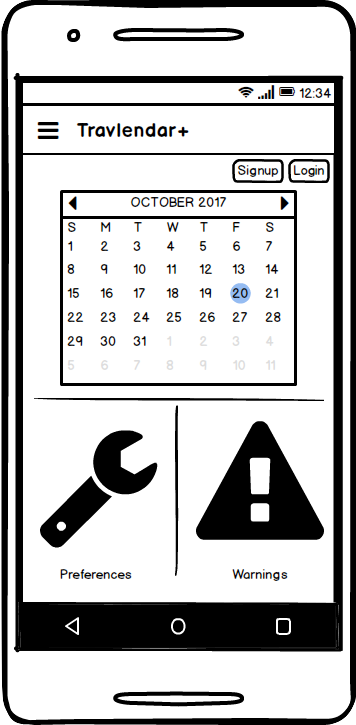
\includegraphics[width=0.7\linewidth]{Homepage.png}
		\caption{Travlendar+ homepage.  
		}
	\label{fig:homepage}
	\begin{center}
		To pursue our aim of realizing a user-friendly and light app, we decided to provide the main functions directly in the homepage. Indeed, from this page, a guest can reach the sign up form, a user can log himself in,can insert a meeting by tapping onto a day in the calendar,can manage his preferences and even access the warnings. \\ 
	\end{center}
	\end{figure}


				
				
	\begin{figure}
	\centering
	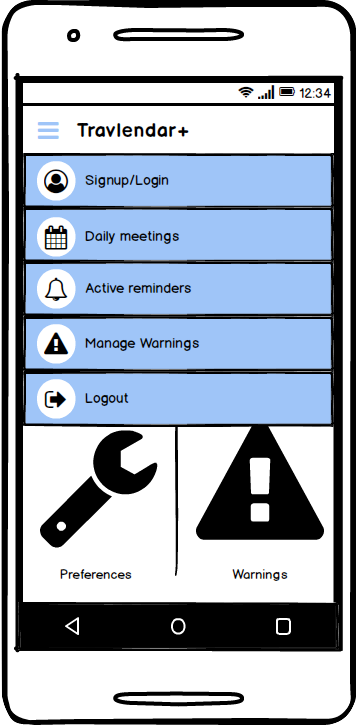
\includegraphics[width=0.7\linewidth]{QuickMenu.png}
	\caption{Quick access menu.}
	\label{fig:quickmenu}
	\begin{center}
		We thought about a quick menu to collect some secondary functions, to make them easily reachable. By tapping on the left high corner of the app. people has the opportunity to either register or log in themselves, to view only the meetings of the current day, to access the reminders they setted up, to manage the warnings and to logout themselves if they are already logged in.
	\end{center}
	\end{figure}

	\begin{figure}
		\centering
		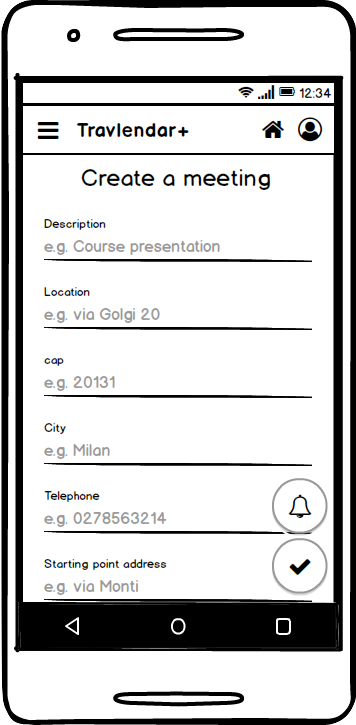
\includegraphics[width=0.7\linewidth]{CreateMeeting.png}
		\caption{Meeting creation page.}
		\label{fig:createmeeting}
		\begin{center}
			This page is a very simple form, which allows the user to finalize the creation of a meeting by filling it in all its fields. 
			The house-logo in the  right corner,on the top band and near the application name, represent the return-to-homepage icon. 
		\end{center}
	\end{figure}

	\begin{figure}
	\centering
	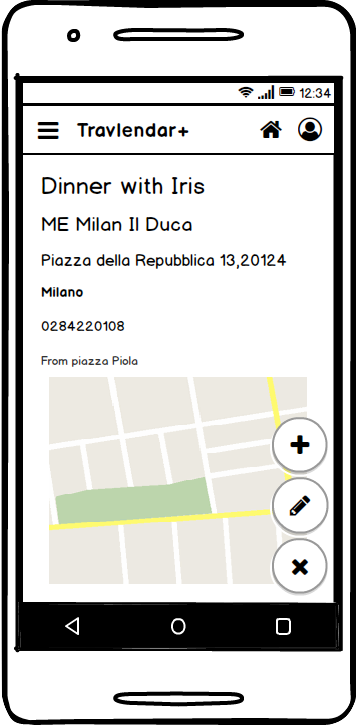
\includegraphics[width=0.7\linewidth]{MeetingView.png}
	\caption{Meeting view page. }
	\label{fig:meeting-view}
	\begin{center}
		This screen wants to provide all the useful information related to a meeting already registered in the system. First details provided, in the highest portion of the page, regard the meeting location and the route to reach the appointment, further information are located below. In addition, on the right part of the screen, there are quick access buttons: the "plus" icon allows the user to add a reminder for the event, the "pencil" icon is to change meeting details and the "x" button provides deletion function. 
	\end{center}
	\end{figure}

	\begin{figure}
		\centering
		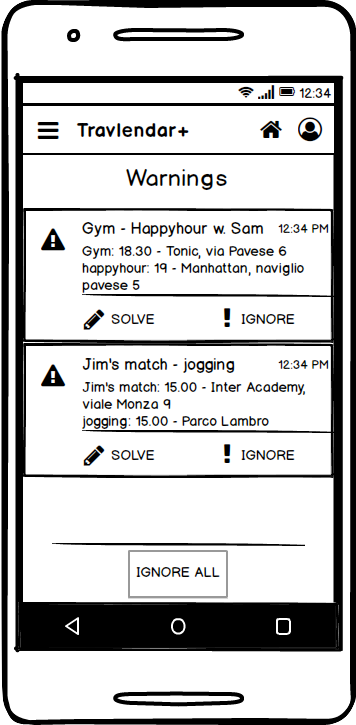
\includegraphics[width=0.7\linewidth]{Warnings.png}
		\caption{Warnings page}
		\label{fig:warnings}
		\begin{center}
			The warnings page has the role to summarize and notify all the conflict among meetings which involv the user's appointments. Every warning is represent by a dialog which points out the meetings that generate the conflict and which has two buttons, one to ignore the warning and other one to solve it by modifying the conflictual meetings. 
			To prevent too much user's clicks, is provided an "ignore all" button, which is equivalent to tap "ignore" for each warning in the list. 
		\end{center}
	\end{figure}

	\begin{figure}
		\centering
		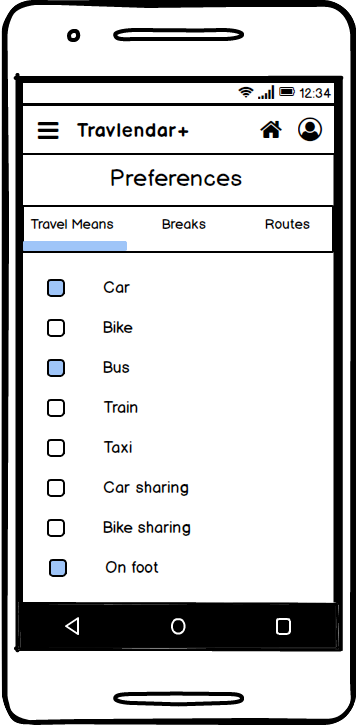
\includegraphics[width=0.7\linewidth]{PreferencesTravelMeans.png}
		\caption{Travel mean preferences page.}
		\label{fig:preferencestravelmeans}
			\begin{center}
			This is a very simple page with a minimalistic design, not to uselessly load the application. However this basical view provides all the function which the user needs to select his preferences on the transports for his travels. 
			Please note that the preference section can be switched by tapping on an specific topic just below the "Preferences" band.
			\end{center}
	\end{figure}

		\begin{figure}
		\centering
		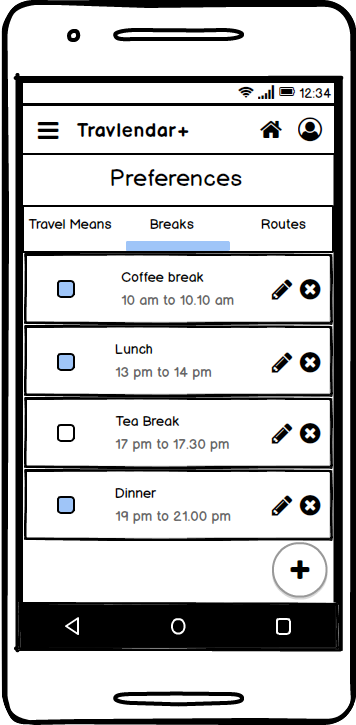
\includegraphics[width=0.7\linewidth]{PreferencesBreaks.png}
		\caption{Break preferences page.}
		\label{fig:preferencesbreaks}
		\begin{center}
			The breaks page consists in a list of events, that represents pauses, organized in order of generation and labeled by the type of the break. For every break are provided both the starting and the ending time, a "pencil" button to allow modifications and a "x" button to remove it. In addition, thanks to the fact that we decided to make the breaks general, that means not related to a specific day, the user has the faculty to either pick or unpick them to activate or deactivate them. 
		\end{center}
		\begin{center}
			
		\end{center}
	\end{figure}
	
		\begin{figure}
		\centering
		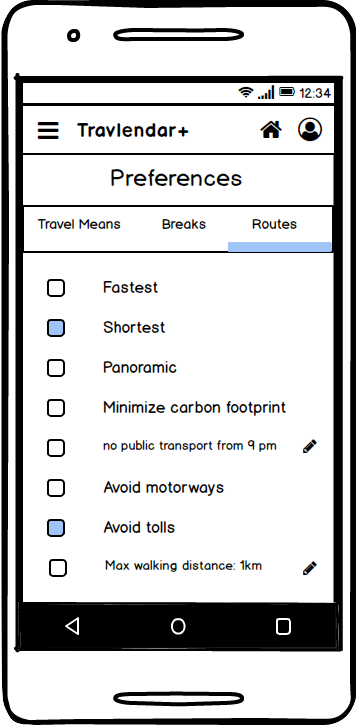
\includegraphics[width=0.7\linewidth]{PreferencesRoutes.png}
		\caption{Route preferences page}
		\label{fig:preferencesroutes}
		\begin{center}
			The route preferences page is very similar to the Travel mean preferences page. The style is the same and the opportunity to pick or unpick elements too, however there are differences. Some of the preferences in this section are mutal exclusive, so the user is prevented to select more than one of them (for instance a user can select either the shortest route or the fastest). Moreover, some selection element has customizable details, they are represented with a pencil logo on the right, and can be managed by the user to best fit his preferences ( for example the user can select after which hour he do not want to use public transports).
		\end{center}
	\end{figure}
	

	
\end{document}

\clearpage
\subsubsection{Software Interfaces}

	Considering the domain of our application, we  decided to integrate in our project some software components to create an easier and more powerful product. 
	\\In order to provide an excellent navigation service, we thought to adopt the Google Maps API, to retrieve the user location through the Google Maps' servers and databases. 
	\\In addition, we noticed that the most complex computations which Travlendar+ should perform are those related to calculating the best route. This idea suggested us to use the APIs of several travel mean sharing services, such as Mobike or CarToGo, 
	to support this crucial phase. We are sure that these APIs are going to allow us to query the databases and to retrive precise information in the quickest and easiest way.
	\\The same reasoning is applicable to forecast, needed to avoid certain routes in case of particular wheater conditions, indeed wheater information from a specific provider are supposed to be rietrieved through its APIs. 
	\\Finally, APIs of public transport societies are required to retrieve real time information about buses,trains and taxis and to mantain the app up to date with relevance to all the related news, for instance about strikes. 
	


\subsection{Non functional requirements}
\begin{itemize}
\item \textbf{Simple User Interface}:
The user interface has to be as simple and intuitive as possible, the application should allow an average user to set up an account and start using the application understanding its functionality in no more than a dozen minutes.

\item \textbf{Portability}: The client has to be compatible to all the major hardware and software platform on the market, this is accomplished using the web application solution presented early.

\item \textbf{Performance}: The application should be able to calculate shortest paths very quickly in order to let the user choose the one that better fits his needs right after setting up the meeting.

\item \textbf{Reliability}: The system should be able to guarantee the service independently of the time, 24/24, 7/7. Thus, the used services should be always available, however, since this is not a critical application, brief unavailability could be acceptable.

\item \textbf{Data integrity, consistency and availability}: System data have to be always accessible. Hence the system should always provide a reliable access to them in normal condition. They also have to be duplicate in order to avoid data losses in case of system fault. 

\item \textbf{Security}: Hashed password should be stored in the database in order to guarantee a high level of privacy to the users. Sensible data such as meetings details will probably be stored locally on the user device, a possible encryption might be considered but it's not a priority
\end{itemize}

\subsection{Scenarios}

\subsubsection{Scenario One}
\begin{table}[htp]
\begin{tabular}{lp{9cm}}
\hline
\bf\large  &\bf\large Creation of an event and Set up of Preferences\\
\hline
\hline

\bf Actors&Jon Snow: habitual user\\
\hline
\bf Flow of events&
As soon as Jon receives  an email from the other members of the Night's Watch, he doesn't wait and, as always, he opens Travlendar+ in order to set up the scheduled the important Meeting for saturday.
He logs into the application inserting his credentials (see use case \autoref{tab:login}) and then from the Homepage he starts creating the new Meeting (see use case \autoref{tab:meetingcreationtab}).
The application suggests an optimal route using the car, as it is the fastest way to get to The Wall from Winterfell where he is currently staying.
Unfortunately, Jon doesn't own a car, nor does he know what a car is, in fact he knows nothing. 
He deletes the Meeting straightaway (see use case \autoref{tab:deletemeetingtab}) and navigates through the app reaching the "Preferences set up" page at once.
Here he deactivates all impossible means of transport (see use case \autoref{tab:activatedeactivatemean}) and leaves as active only On Foot and By Horse options.
He then recreates the exact same Meeting as before and this time the system comes up with a feasible travel.
Satisfied, Jon closes the app and goes on hunting rabbits. 



\end{tabular}
\caption{Scenario 1} 
\label{tab:scenarioone}
\end{table}

\clearpage
\subsubsection{Scenario Two}
\begin{table}[htp]
\begin{tabular}{lp{9cm}}
\hline
\bf\large  &\bf\large Warning Solving and Reminder Addition\\
\hline
\hline

\bf Actors&Jon Snow: habitual user\\
\hline
\bf Flow of events&
The following day, a raven from Dragonstone arrives at Winterfell, Jon's heart starts beating faster as soon as he notices the Targaryen sigil.
It's Danaerys who is asking for a date with him on saturday night.
Jon, unable to decide whether he can make it for both the appointments on time, lets his favourite companion decide it for him.
He starts up Travlendar+ and creates the meeting (see use case \autoref{tab:meetingcreationtab}).
Unfortunately, the ride from Dragonstone to The Wall is long, and a warning appears on Jon's app stating that he is not going to be able to make it on time for both the meetings and a reschedule proposal is made. 
Jon Solves the conflict (see use case \autoref{tab:warningsolving}) and the warning disappears.
Since he was longing for a date with Dany, Jon decides to add a Reminder (see use case \autoref{tab:reminderaddition}) to the event in order for him to have enough time to suit up for the special date.



\end{tabular}
\caption{Scenario 1} 
\label{tab:scenarioone}
\end{table}

\clearpage
\subsection{Use Cases}
This section contains all the use cases initially described with the use cases UML model of the whole system.

\subsubsection{User Page use cases}
\begin{figure}[htp] 

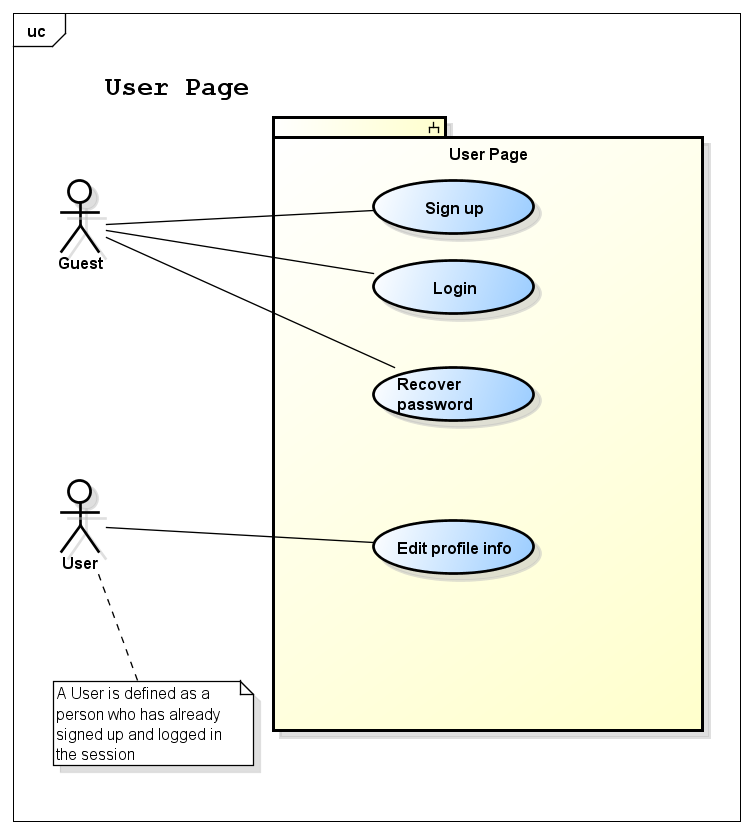
\includegraphics[width=\textwidth]{usecases/png/userpage} 
\caption{Use cases relative to the user registration and authentication} 
\label{fig:userpage} 
\end{figure} 

\newpage
\subsubsection{Sign up}

\begin{table}[htp]

\begin{tabular}{r|p{7cm}}
\bf\large Name&\bf\large Sign up\\
\hline
\hline
\bf Actors&Guest\\
\hline
\bf Entry conditions&None\\
\hline
\bf Flow of events&
\begin{itemize}
\item The guest reaches the registration page containing the relative form
\item The guest fills up the form and clicks on "Sign up" to complete the process
\item The system redirects the user to his profile page and sends a confirmation email.
\end{itemize}
\\
\hline
\bf Exit conditions&The guest has successfully registered in the system. \\
\hline
\bf Exceptions&The guest left an empty field or typed
 something wrong an error message is displayed 
 and the user is asked to fill the form again.\\
\hline

\end{tabular}
\caption{Sign up Use Case table} \label{tab:signup}
\end{table}


 \newpage
\subsubsection{Login}
\begin{table}[htp]

\begin{tabular}{r|p{7cm}}
\bf\large Name&\bf\large Login\\
\hline
\hline
\bf Actors&User\\
\hline
\bf Entry conditions&The user has already registered.\\
\hline
\bf Flow of events&
\begin{itemize}
\item The user reaches the login page containing the relative form
\item The user types the username and password in the login form and click on "Login" button.
\item The system redirects the user to the application homepage.
\end{itemize}
\\
\hline
\bf Exit conditions&The user has access to the application functionalities. \\
\hline
\bf Exceptions&Username and password didn't correspond or the username didn't exist ,an error message is displayed and the user is asked to fill the login form again.\\
\hline

\end{tabular}

\caption{This is my one big table } \label{tab:login}
%\autoref{fig:userpage}
\end{table}
\newpage
\subsubsection{Password Recovery}
\begin{table}[htp]
\begin{tabular}{r|p{7cm}}
\bf\large Name&\bf\large Recover Password \\
\hline
\hline
\bf Actors&User\\
\hline
\bf Entry conditions&The user has already registered.\\
\hline
\bf Flow of events&
\begin{itemize}
\item The user reaches the login page containing the relative form
\item The user clicks on "Password recovery" button and is redirected to the password recovery page.
\item The user inserts his email and clicks on "reset password".
\item The system sends an email to the user with a link and instruction to reset the password.
\item The user chooses and types a new password and confirms.
\item The system redirects the user to the login page.
\end{itemize}
\\
\hline
\bf Exit conditions&The user has changed his password \\
\hline
\bf Exceptions&The inserted email doesn't match any user in the database, it is displayed an error message and the user is asked to retype a valid email.\\
\hline

\end{tabular}
\caption{Recover password Use Case table} \label{tab:recoverpassword}
\end{table}


\newpage
\subsubsection{Schedule Management use cases}
\begin{figure}[htp] 
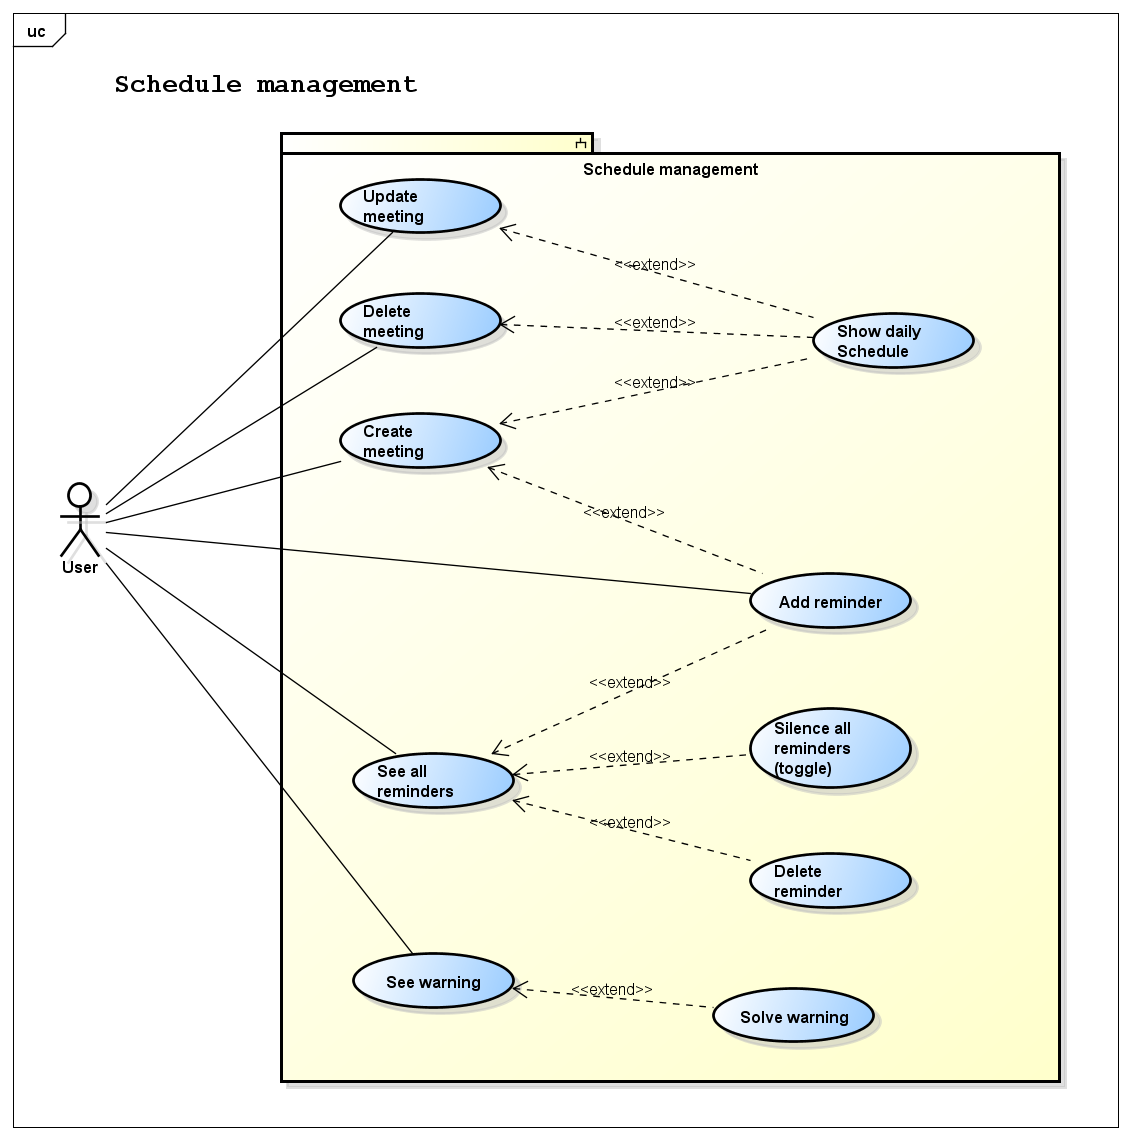
\includegraphics[width=\textwidth]{usecases/png/schedulemanagement} 
\caption{Main use cases showing the functionalities of Travlendar+ application relative to the meetings creation and management} 
\label{fig:schedulemanagement} 
\end{figure}

\newpage
\subsubsection{Meeting Creation}
\begin{table}[htp]

\begin{tabular}{r|p{7cm}}
\bf\large Name&\bf\large Creation of a meeting\\
\hline
\hline
\bf Actors&User\\
\hline
\bf Entry conditions&The user is logged in and is in the main page.\\
\hline
\bf Flow of events&
\begin{itemize}

\item The user clicks on "Create meeting" button and he is redirected to the page with the input form to create a meeting.

\item The user fills up the form with the meeting information (title, location, description, date and time, flags, etc...).

\item The system checks whether the meeting at the specified time and date is possible according to the user preferences and the current daily schedule, the optimal route is proposed.


\item The user is then redirected to the main page.

\end{itemize}
\\
\hline
\bf Exit conditions&The new meeting with the calculated optimal route is added to the user Calendar. In the case of the incompatibility of a meeting with others a warning is created.\\
\hline
\bf Exceptions&The information inserted is wrong or some information is missing: a corresponding error is displayed and the user is asked to modify the inserted information accordingly.
\\
\hline

\end{tabular}
\caption{Meeting Creation Use Case table}
 \label{tab:meetingcreationtab}
\end{table}
\newpage
\subsubsection{Reminder Addition}
\begin{center}
\begin{tabular}{r|p{7cm}}
\bf\large Name&\bf\large Addition of a reminder\\
\hline
\hline
\bf Actors&User\\
\hline
\bf Entry conditions&The user is logged in and is on the page of a meeting\\
\hline
\bf Flow of events&
\begin{itemize}
\item The user clicks on "Add reminder" button and he is redirected to the page with the input form to add a reminder.

\item The user fills up the form with the type of reminder and the time he wants to be reminded of the upcoming meeting.

\item  The system adds the reminder and the user is redirected to the relative meeting page.

\end{itemize}
\\
\hline
\bf Exit conditions&The reminder is added to the meeting \\
\hline
\bf Exceptions&There exists already an identical reminder and it is not added to the meeting\\
\hline

\end{tabular}
\end{center}
\newpage
\subsubsection{Warning Solving}
\begin{center}
\begin{tabular}{r|p{7cm}}
\bf\large Name&\bf\large Solving a warning\\
\hline
\hline
\bf Actors&User\\
\hline
\bf Entry conditions&The user is logged in and is in the page of a warning\\
\hline
\bf Flow of events&
\begin{itemize}
\item The user clicks on "Solve warning" button and he is redirected to a page that lets him
choose how to solve the conflict: the timing of two overlapping meetings can be changed, or one of the two meetings has to be canceled; 
\item  The user solves the conflict the way he wants and clicks on the button "Done".
\item  The system checks whether the conflict has been solved and the user is redirected to the warnings page.
\end{itemize}
\\
\hline
\bf Exit conditions&The warning has been solved and is deleted from the system and from the list of warnings in the corresponding page\\
\hline
\bf Exceptions&The warning was not solved after the user's modifications, the unresolved warning will still be present and a message stating that the conflict wasn't successfully solved is displayed. The user is redirected to the warning page.
\\
\hline

\end{tabular}
\end{center}


\newpage
\subsubsection{User Preferences use cases}
\begin{figure}[htp]
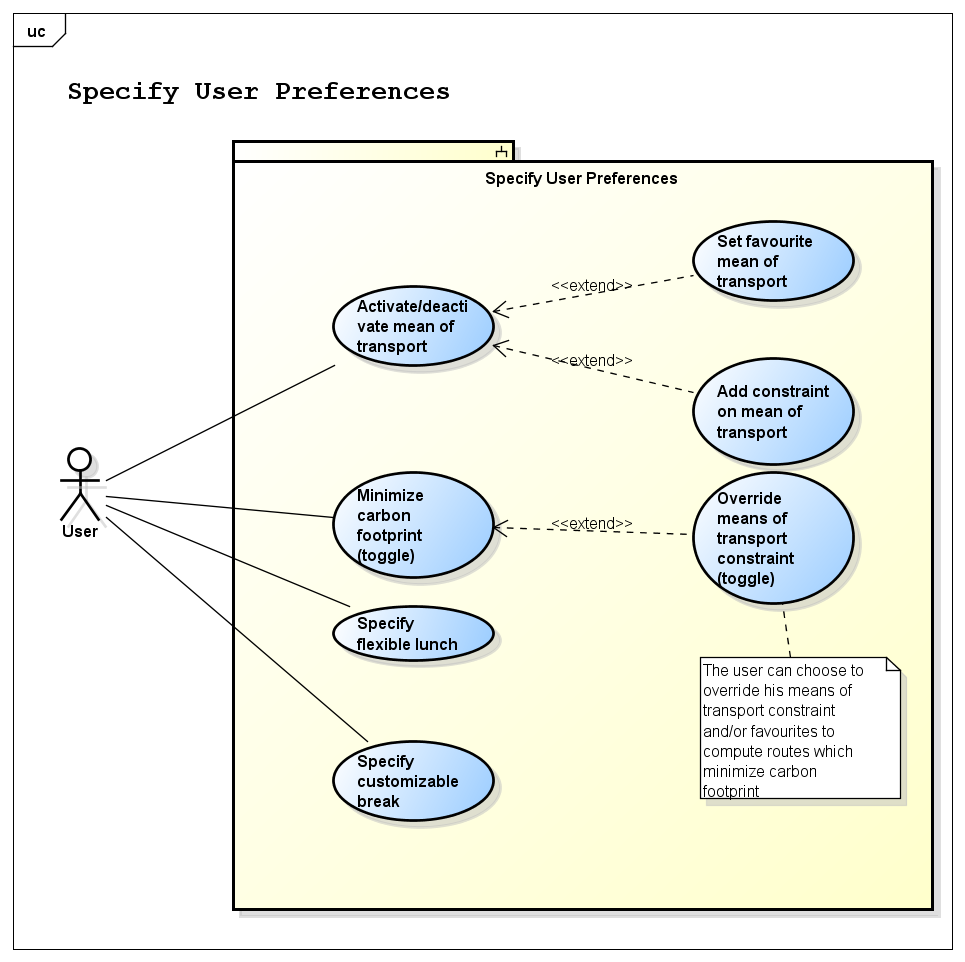
\includegraphics[width=\textwidth]{usecases/png/specifyuserpreferences} 
\caption{Use cases showing the user preferences and relative functonalities} 
\label{fig:specifyuserpreferences} 
\end{figure}

\newpage
\subsubsection{Means activation/deactivation}
\begin{table}
\begin{tabular}{r|p{7cm}}
\bf\large Name&\bf\large Activate/deactivate mean of transport\\
\hline
\hline
\bf Actors&User\\
\hline
\bf Entry conditions&The user is logged in and is in the user preferences page\\
\hline
\bf Flow of events&
\begin{itemize}
\item The user clicks on "Choose means of transport" button and he is redirected to a page containing a list of all possible means of transport;
\item  The user unflags all the means of transport he does not intend to use.
\item  The user clicks on "Done" button and is redirected to the user preferences page.
\end{itemize}
\\
\hline
\bf Exit conditions&The unflagged means of transport are removed from the possible means needed to compute a route\\
\hline
\bf Exceptions&The user unselected every mean of transport, clicking "Done" button has no effect and an error message stating that at lest one mean of trasport has to be flagged.
\\
\hline

\end{tabular}
\caption{This is my one big table} \label{tab:activatedeactivatemean}
\end{table}





\clearpage
\subsection{Activity Diagrams}

\subsubsection{Meeting creation process}
Whenever the user fills up the form relative to creation of a meeting and presses "Create meeting" the system does what is visually described in the diagram.
\\It checks for conflicts while asynchronously queries public transport providers, when the data gets back and the meeting is set as regular or is put in a warning with other meetings the meeting is created and the process is done.

\begin{figure}[htp] 

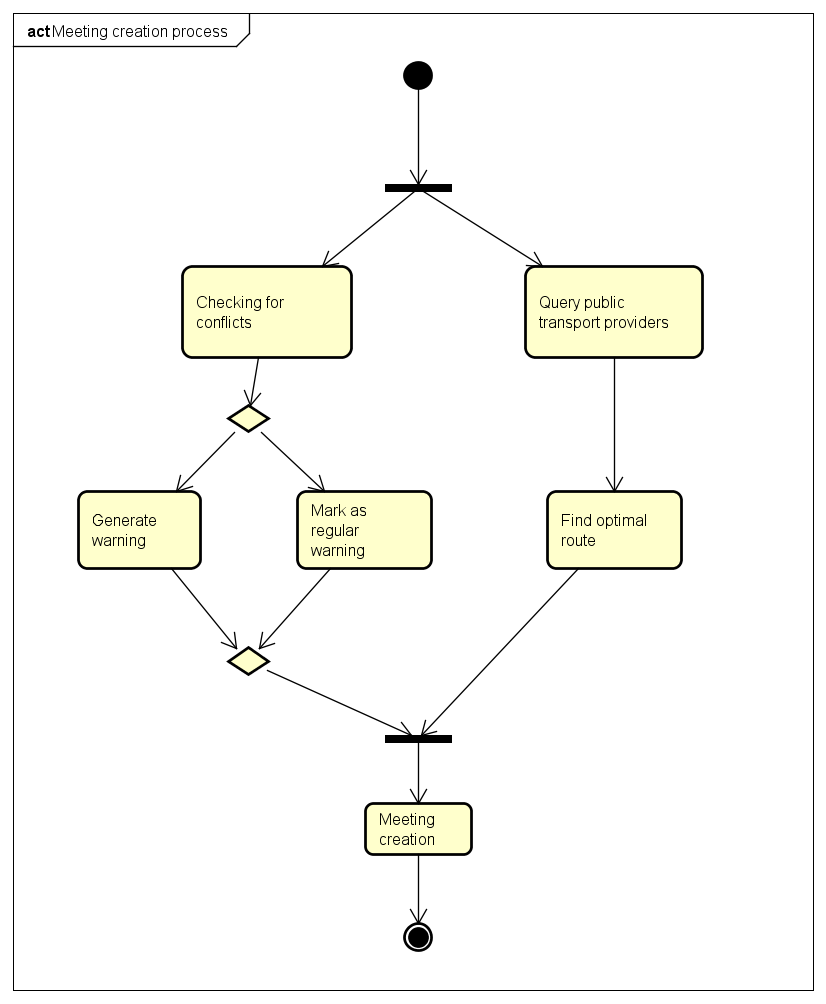
\includegraphics[width=\textwidth]{activitydiagrams/meetingcreationprocess} 
\caption{This diagram shows the activities carried out by the system in the meeting creation process} 
\label{fig:meetingcreationprocess} 
\end{figure} 


\clearpage
\subsection{State Charts}

\subsubsection{Meeting State Machine}
This State Machine was created with the purpose to identify the various states a meeting can be in and the show the transition events that modify its state.

\begin{figure}[htp] 

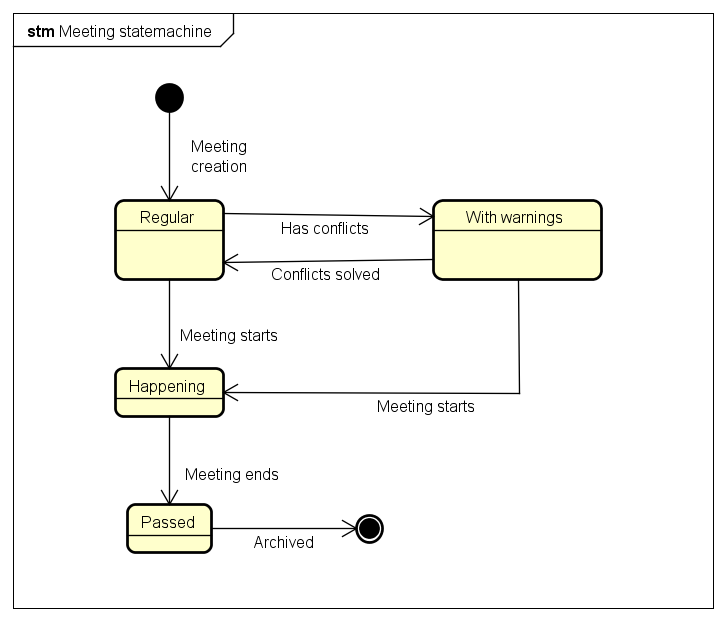
\includegraphics[width=\textwidth]{statecharts/meetingstatemachine} 
\caption{State Chart showing states of a meeting} 
\label{fig:meetingstatemachine} 
\end{figure} 

\newpage
\subsubsection{Basic UX State Chart}
We provide a simple and basic User Experience State Chart which highlights the different pages a user can find himself in (and the System redirects the user to, when an event happens). 
\\We believe this could be helpful to understand and visualize the entire application.

\begin{figure}[htp] 

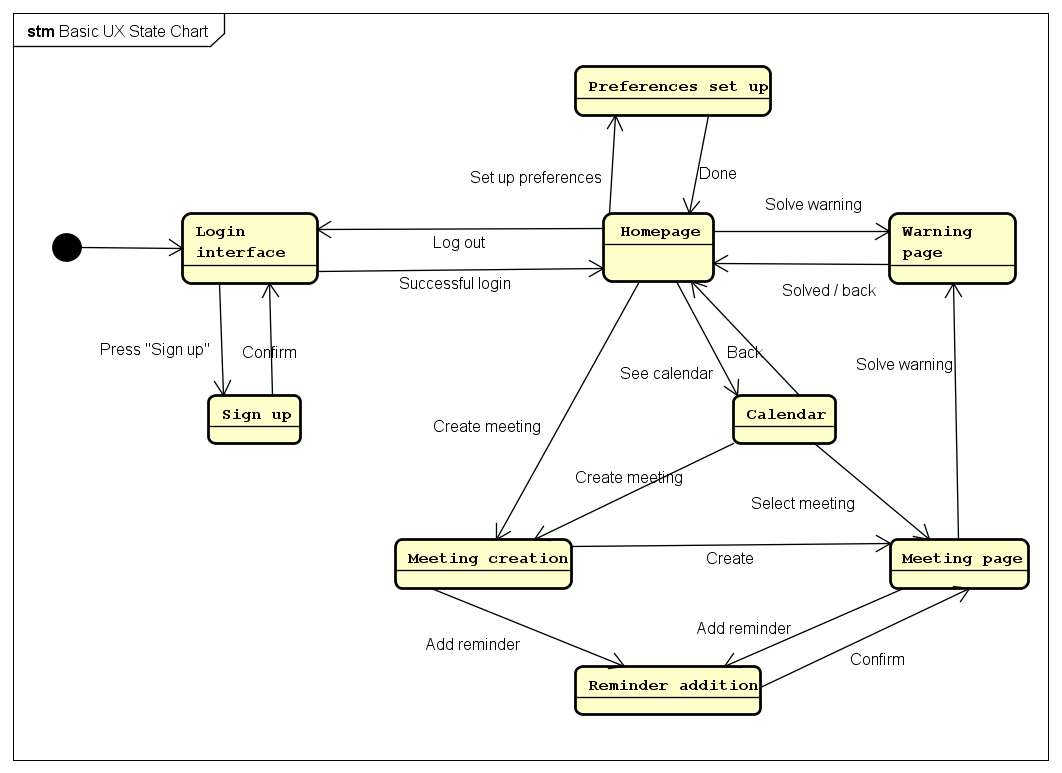
\includegraphics[width=\textwidth]{statecharts/basicux} 
\caption{A basic User eXperience chart of the application} 
\label{fig:ux} 
\end{figure}

\clearpage
\subsection{Sequence Diagrams}
\subsubsection{Signup/Login Sequence Diagram}

This sequence diagram points out the steps to make a proper signup and to correctly login to Travlendar+ as a specific
user. As you can see, there are three main phases, fulfilling the registration form, verifying the user email and logging in. 
In order to mark up the differences between  registered and  unregistered customers, we called them respectively 'user' and 'guest'. 
Clearly, the email verification leads to an automatic login, thus the system redirects the user to his personal page. This also explain why we inserted logout before the login step. 

\begin{figure}[htp]
	
	\centering
	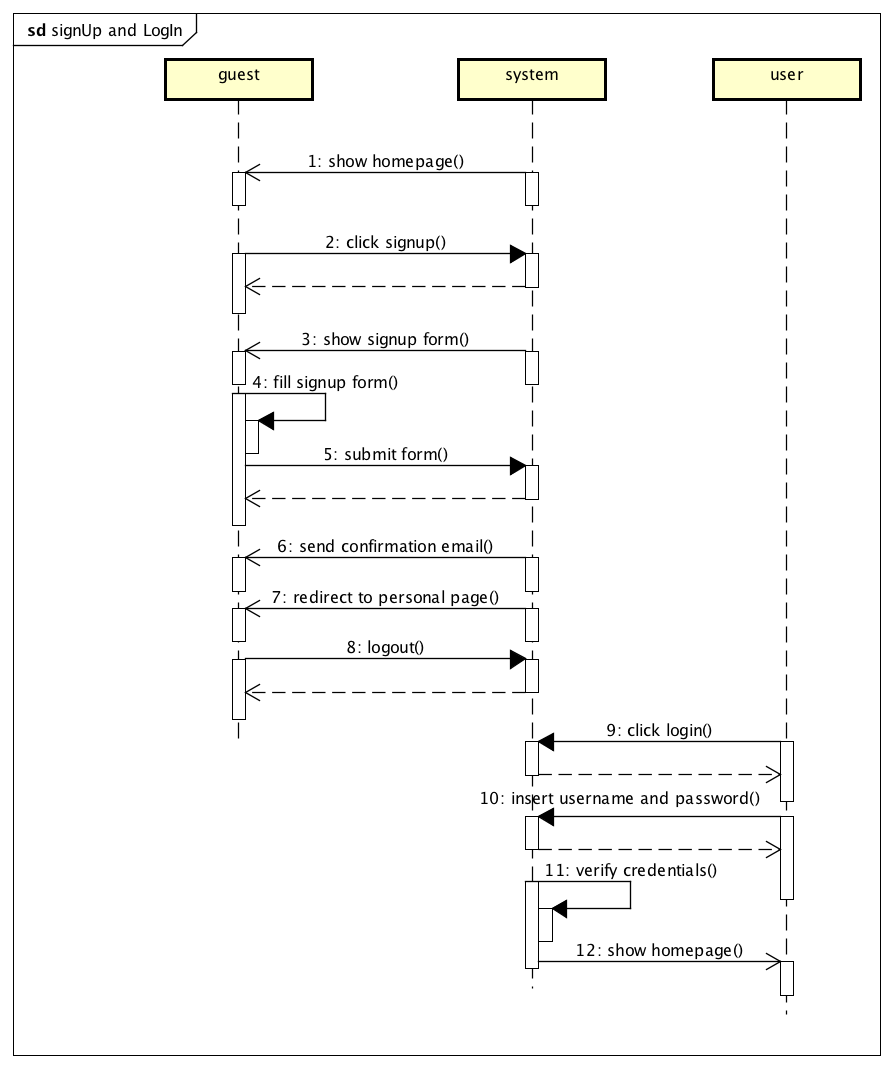
\includegraphics[width=\textwidth]{sequencediagrams/signup-logIn}
	\caption{The sequence diagram about Signup and Login operations.}
	\label{fig:signup-login} 

\end{figure}
\newpage

\subsubsection{Meeting Creation Sequence Diagram}

This sequence diagram explains how to create a meeting, assuming that the operation is accomplished properly.
Oppositely,in case of failures such as trying to insert a duplicate meeting, Travlendar+ prevents the appointment registration. 
As the chart shows, when a user selects a date on the calendar, the system provides him a meeting form, where he can insert all the required information. Then, the app enters in an intense computational phase. In addition to the local operations such as verifying overlappings and analyzing preferences, during this step Travlendar+ also interacts with external systems. 
We labeled them as 'service providers' referring for example to the public transports server, a forecast agency infrastructure, sharing services systems etc, and we suppose the related events to be database queries. 
The entire process ends with the registration of the event into the system and a positive notification to the user. 

\begin{figure}[htp]
	
	\centering
	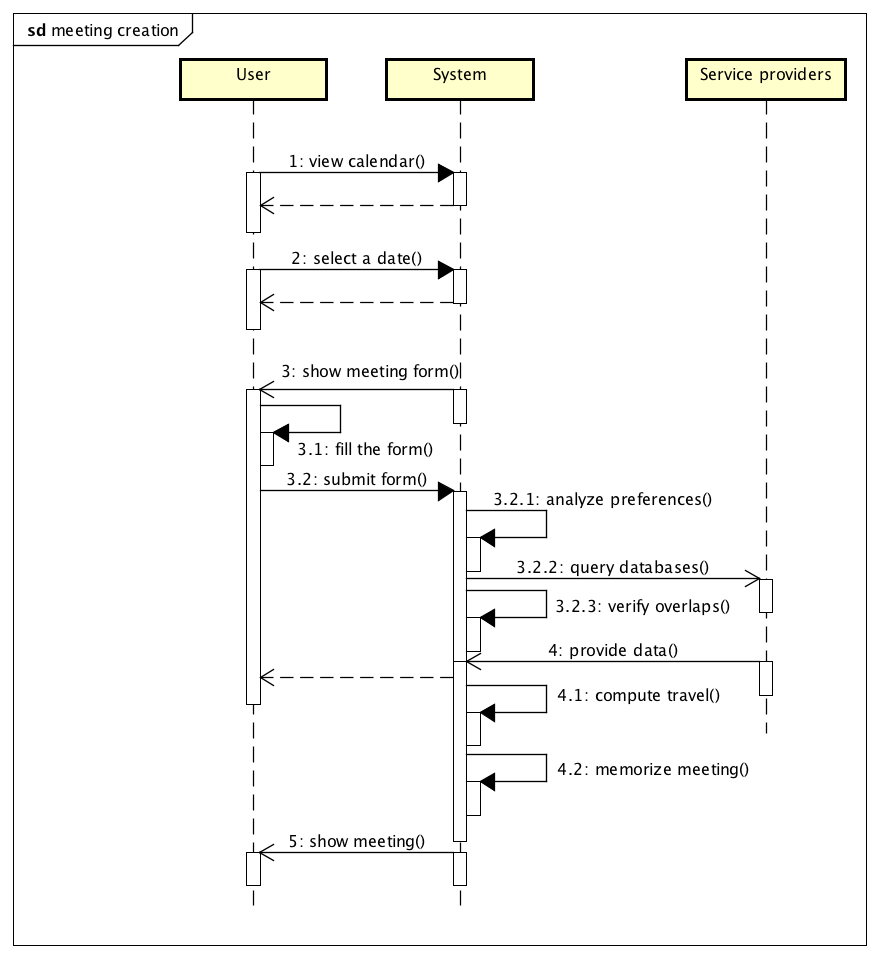
\includegraphics[width=\textwidth]{sequencediagrams/meetingcreation}
	\caption{The sequence diagram about the process flow of a meeting creation.}
	\label{fig:meetingcreation}
		
\end{figure}
\newpage

\subsubsection{Warnings Solving Sequence Diagram}

The last two sequence diagrams refer to the user reaction against the generation of a warning by the system. 
In order to model correctly the two possibile user choices, we have done two diagrams, one for each possibility. 
The first and simple chart explains what happens if the user decides to ignore a warning, that is just the deletion of the notification, because we assume his specific intention not to consider it. 
The second diagram, quite more complex, regards the warning resolution through an event rescheduling made by the user. For this reason, Travlendar+ allows to directly go from the warning to the conflictual meetings, in order to modify them. 
Obviously, considering that a conflict, same as a warning, can involve from two up to a huge number of appointments, it is clear that the operation number 5 could be done for more than just one meeting involved in the conflict. 

\begin{figure}[htp]
	\centering
	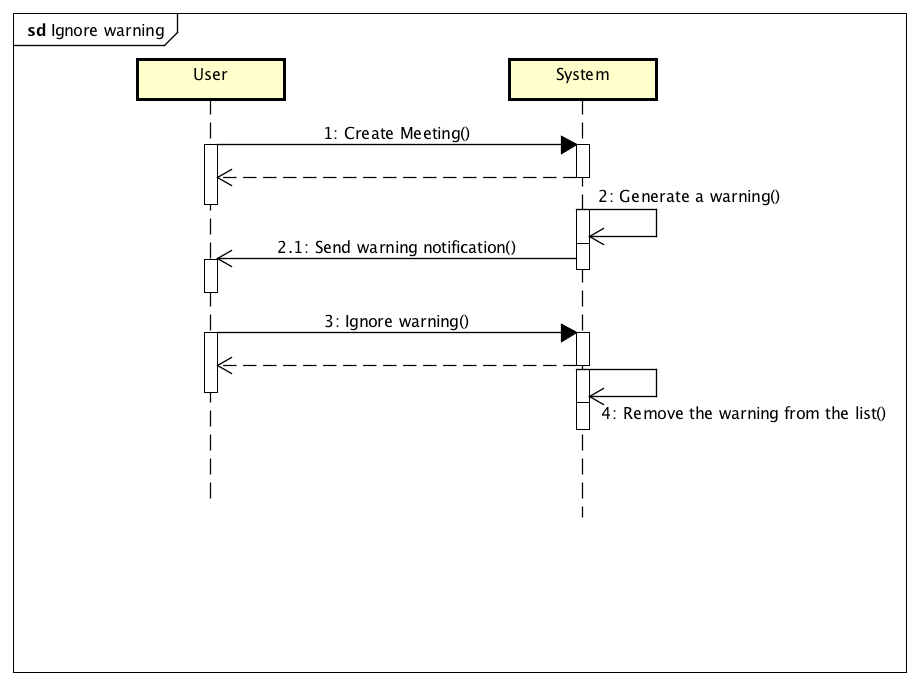
\includegraphics[width=\textwidth]{sequencediagrams/Ignorewarning}
	\caption{The sequence diagram that shows the steps to ignore a warning.}
	\label{fig:ignorewarning}
\end{figure}

\begin{figure}[htp]

	\centering
	\includegraphics[width=\textwidth]{"sequencediagrams/ warningresolution"}
	\caption{the sequence diagram that shows how to solve a warning.}
	\label{fig:-warningresolution}
	\begin{center}

	\end{center}
\end{figure}
\newpage




\clearpage
\subsection{Class Diagram}

	In order to convey detailed and clear information, we provide a high-level representation of Travlendar+ skeleton of the software side, however this is just a first sketch that will be enriched and improved or even changed in the design document. \\



\begin{figure}[htp] 

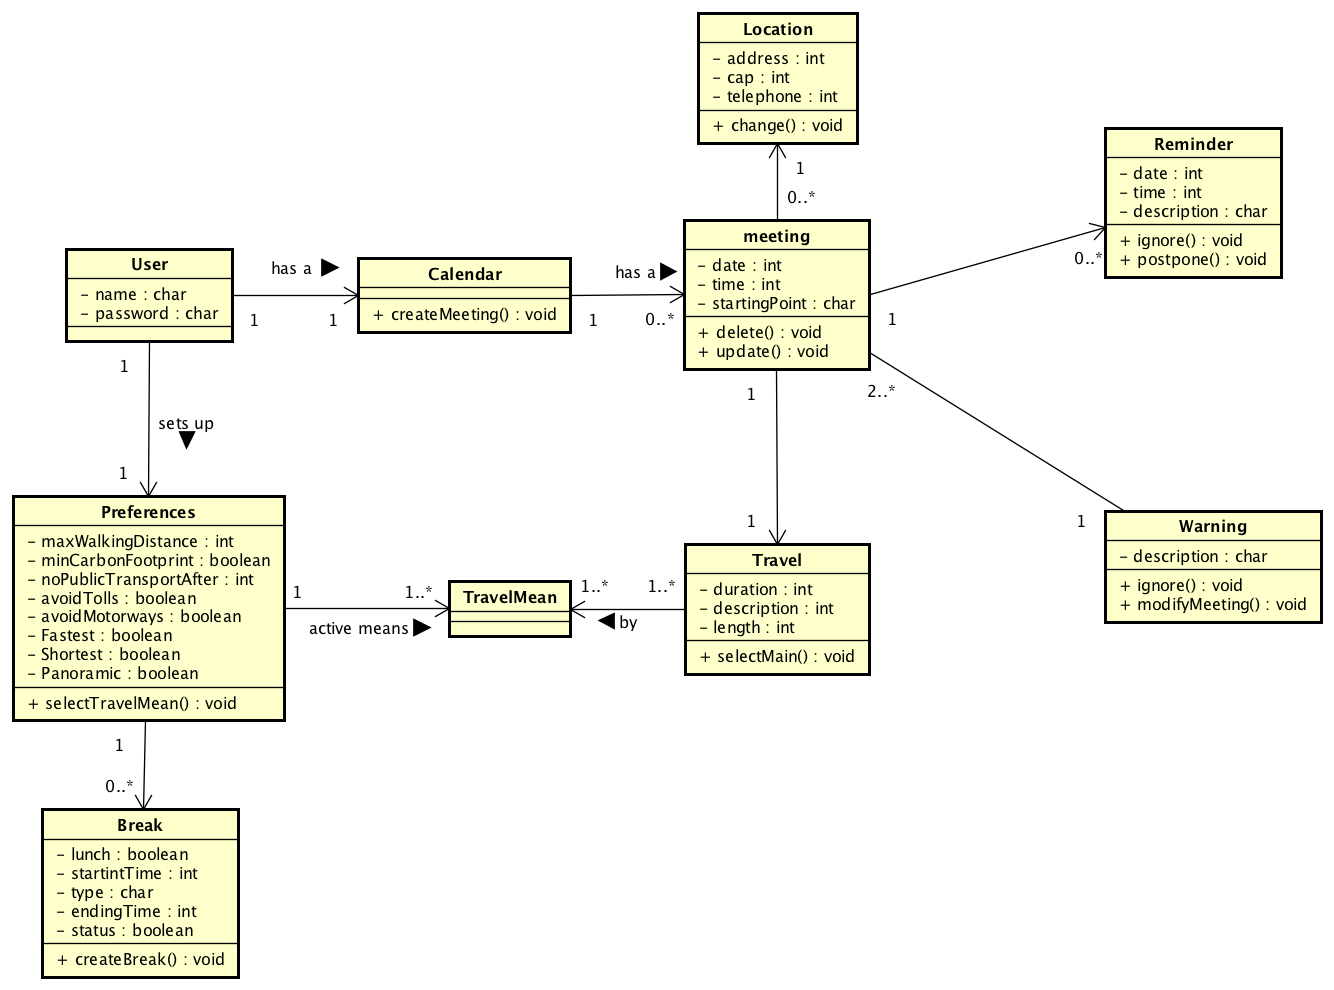
\includegraphics[width=\textwidth]{classdiagrams/ClassDiagramTravlendar+} 
\caption{Travlendar+ class diagram} 
\label{fig:ux} 
\end{figure}


\clearpage
\section{Formal Analysis using Alloy}
\subsection{Model}

\texttt{\-     \ \ 1    \qquad {\color{green}/{\color{green}/****************SIGNATURES*****************/}/}\\
\-     \ \ 2    \qquad \\
\-     \ \ 3    \qquad {\color{blue}abstract} {\color{blue}sig} Boolean \{\\
\-     \ \ 4    \qquad \\
\-     \ \ 5    \qquad \}\\
\-     \ \ 6    \qquad \\
\-     \ \ 7    \qquad {\color{blue}one} {\color{blue}sig} true {\color{blue}extends} Boolean \{ \}\\
\-     \ \ 8    \qquad \\
\-     \ \ 9    \qquad {\color{blue}one} {\color{blue}sig} false {\color{blue}extends} Boolean \{ \}\\
\-    \ 10      \qquad \\
\-    \ 11      \qquad \\
\-    \ 12      \qquad {\color{blue}sig} Travel \{\\
\-    \ 13      \qquad \-\qquad means: {\color{blue}set} TravelMean\\
\-    \ 14      \qquad \}\\
\-    \ 15      \qquad \\
\-    \ 16      \qquad {\color{blue}abstract} {\color{blue}sig} TravelMean \{ \}\\
\-    \ 17      \qquad \\
\-    \ 18      \qquad {\color{blue}one} {\color{blue}sig} Car {\color{blue}extends} TravelMean \{\\
\-    \ 19      \qquad \\
\-    \ 20      \qquad \}\\
\-    \ 21      \qquad \\
\-    \ 22      \qquad {\color{blue}one} {\color{blue}sig} SharedCar {\color{blue}extends} TravelMean \{ \}\\
\-    \ 23      \qquad \\
\-    \ 24      \qquad {\color{blue}one} {\color{blue}sig} Bike {\color{blue}extends} TravelMean \{ \}\\
\-    \ 25      \qquad \\
\-    \ 26      \qquad {\color{blue}one} {\color{blue}sig} SharedBike {\color{blue}extends} TravelMean \{ \}\\
\-    \ 27      \qquad \\
\-    \ 28      \qquad {\color{blue}one} {\color{blue}sig} Train {\color{blue}extends} TravelMean \{ \}\\
\-    \ 29      \qquad \\
\-    \ 30      \qquad {\color{blue}one} {\color{blue}sig} Metro {\color{blue}extends} TravelMean \{ \}\\
\-    \ 31      \qquad \\
\-    \ 32      \qquad {\color{blue}one} {\color{blue}sig} Bus {\color{blue}extends} TravelMean \{ \}\\
\-    \ 33      \qquad \\
\-    \ 34      \qquad {\color{blue}one} {\color{blue}sig} OnFoot {\color{blue}extends} TravelMean \{ \}\\
\-    \ 35      \qquad \\
\-    \ 36      \qquad {\color{blue}sig} Preferences \{\\
\-    \ 37      \qquad \-\qquad minimizeCarbonFootprint: {\color{blue}one} Boolean,\\
\-    \ 38      \qquad \-\qquad breaks: {\color{blue}set} Break,\\
\-    \ 39      \qquad \-\qquad activeMeansOfTransport: TravelMean -> {\color{blue}one} Boolean\\
\-    \ 40      \qquad \}\{\\
\-    \ 41      \qquad \-\qquad  {\color{green}// A {\color{blue}set} of preferences must refers only to {\color{blue}one} user}\\
\-    \ 42      \qquad \-\qquad {\color{blue}one} u:User | this = u.preferences\\
\-    \ 43      \qquad \}\\
\-    \ 44      \qquad \\
\-    \ 45      \qquad {\color{blue}sig} Break \{\\
\-    \ 46      \qquad \-\qquad active: {\color{blue}one} Boolean,\\
\-    \ 47      \qquad \-\qquad lunch: {\color{blue}one} Boolean\\
\-    \ 48      \qquad \}\\
\-    \ 49      \qquad \\
\-    \ 50      \qquad {\color{blue}sig} User \{\\
\-    \ 51      \qquad \-\qquad calendar: {\color{blue}one} Calendar,\\
\-    \ 52      \qquad \-\qquad preferences: {\color{blue}one} Preferences\\
\-    \ 53      \qquad  \}\\
\-    \ 54      \qquad \\
\-    \ 55      \qquad {\color{blue}sig} Calendar \{\\
\-    \ 56      \qquad \-\qquad meetings: {\color{blue}set} Meeting\\
\-    \ 57      \qquad \}\{\\
\-    \ 58      \qquad \-\qquad  {\color{green}// A calendar must refers only to {\color{blue}one} user}\\
\-    \ 59      \qquad \-\qquad {\color{blue}one} u:User | this = u.calendar\\
\-    \ 60      \qquad \}\\
\-    \ 61      \qquad \\
\-    \ 62      \qquad {\color{blue}sig} Reminder \{\\
\-    \ 63      \qquad \\
\-    \ 64      \qquad \}\\
\-    \ 65      \qquad \\
\-    \ 66      \qquad {\color{blue}sig} Location \{\\
\-    \ 67      \qquad \\
\-    \ 68      \qquad \}\\
\-    \ 69      \qquad \\
\-    \ 70      \qquad {\color{blue}sig} Meeting \{\\
\-    \ 71      \qquad \-\qquad location: {\color{blue}one} Location,\\
\-    \ 72      \qquad \-\qquad route: {\color{blue}one} Travel,\\
\-    \ 73      \qquad \-\qquad next: {\color{blue}lone} Meeting,\\
\-    \ 74      \qquad \-\qquad previous: {\color{blue}lone} Meeting,\\
\-    \ 75      \qquad \-\qquad reminders: {\color{blue}set} Reminder,\\
\-    \ 76      \qquad \-\qquad status: {\color{blue}one} MeetingState,\\
\-    \ 77      \qquad \-\qquad warning: {\color{blue}lone} Warning,\\
\-    \ 78      \qquad \-\qquad conflict: {\color{blue}set} Meeting,\\
\-    \ 79      \qquad \-\qquad weather: {\color{blue}one} WeatherForecast\\
\-    \ 80      \qquad \} \\
\-    \ 81      \qquad \\
\-    \ 82      \qquad {\color{blue}abstract} {\color{blue}sig} MeetingState \{\\
\-    \ 83      \qquad  \\
\-    \ 84      \qquad \}\\
\-    \ 85      \qquad \\
\-    \ 86      \qquad {\color{blue}one} {\color{blue}sig} Regular {\color{blue}extends} MeetingState\{ \}\\
\-    \ 87      \qquad \\
\-    \ 88      \qquad {\color{blue}one} {\color{blue}sig} WithWarning {\color{blue}extends} MeetingState\{ \}\\
\-    \ 89      \qquad \\
\-    \ 90      \qquad {\color{blue}one} {\color{blue}sig} Happening {\color{blue}extends} MeetingState\{ \}\\
\-    \ 91      \qquad \\
\-    \ 92      \qquad {\color{blue}one} {\color{blue}sig} Passed {\color{blue}extends} MeetingState\{ \}\\
\-    \ 93      \qquad \\
\-    \ 94      \qquad {\color{blue}abstract} {\color{blue}sig} WeatherForecast \{\\
\-    \ 95      \qquad \\
\-    \ 96      \qquad \}\\
\-    \ 97      \qquad \\
\-    \ 98      \qquad {\color{green}//This symbolizes every case of 'good' weather (e.g. Cloudy, Partially Cloudy, etc.)}\\
\-    \ 99      \qquad {\color{blue}one} {\color{blue}sig} Sunny {\color{blue}extends} WeatherForecast\{ \}\\
\-   100        \qquad \\
\-   101        \qquad {\color{green}//This symbolizes every case of 'bad' weather (e.g. Snowy, Stormy, extremely Windy, etc.)}\\
\-   102        \qquad {\color{blue}one} {\color{blue}sig} Rainy {\color{blue}extends} WeatherForecast \{ \}\\
\-   103        \qquad \\
\-   104        \qquad {\color{green}//doppia freccia tra meeting e warning}\\
\-   105        \qquad \\
\-   106        \qquad {\color{blue}sig} Warning \{\\
\-   107        \qquad \-\qquad conflicts: {\color{blue}set} Meeting\\
\-   108        \qquad \} \{\\
\-   109        \qquad {\color{green}//meetings set has to be at least >=2 \qquad otherwise the conflict wouldn't exist}\\
\-   110        \qquad \-\qquad \#conflicts > 1\\
\-   111        \qquad \}\\
\-   112        \qquad \\
\-   113        \qquad {\color{green}//problema: tutti i meeting nella stessa location}\\
\-   114        \qquad \\
\-   115        \qquad {\color{green}/{\color{green}/****************CONSTRAINTS*****************/}/}\\
\-   116        \qquad \\
\-   117        \qquad {\color{green}//-----------------MEETING STATUS CONSTRAINTS}\\
\-   118        \qquad \\
\-   119        \qquad {\color{green}//The status=With Warning implies that there is a Warning}\\
\-   120        \qquad {\color{blue}fact} \{\\
\-   121        \qquad \-\qquad {\color{blue}all} m:Meeting | m.status=WithWarning {\color{blue}implies} \#m.warning=1\\
\-   122        \qquad \}\\
\-   123        \qquad \\
\-   124        \qquad {\color{green}//Every Meeting with a warning must have their status set to With Warning}\\
\-   125        \qquad {\color{blue}fact} \{\\
\-   126        \qquad \-\qquad {\color{blue}all} w:Warning | {\color{blue}all} m:w.conflicts | m.status=WithWarning\\
\-   127        \qquad \}\\
\-   128        \qquad \\
\-   129        \qquad {\color{green}//If the status is Regular, Happening or passed, the Meeting does not have any Warning}\\
\-   130        \qquad {\color{blue}fact} \{\\
\-   131        \qquad \-\qquad {\color{blue}all} m:Meeting | (m.status=Regular {\color{blue}or} m.status=Passed {\color{blue}or} m.status=Happening ) \\
\-   132        \qquad \-\qquad \-\qquad \-\qquad \-\qquad   {\color{blue}implies} \#m.warning=0\\
\-   133        \qquad \}\\
\-   134        \qquad \\
\-   135        \qquad {\color{green}//-----------------------CARDINALITY CONSTRAINTS}\\
\-   136        \qquad \\
\-   137        \qquad {\color{green}//Function to retrieve the Calendar owner}\\
\-   138        \qquad {\color{blue}fun} calendarOwner[c: Calendar]: {\color{blue}set} User \{\\
\-   139        \qquad \-\qquad \{u: User | u.calendar = c\}\\
\-   140        \qquad \}\\
\-   141        \qquad \\
\-   142        \qquad {\color{green}//A User can only have one Calendar}\\
\-   143        \qquad {\color{blue}fact} OneCalendarPerUser\{ \\
\-   144        \qquad \-\qquad {\color{blue}no} disj c1,c2: Calendar | {\color{blue}all} u:User | c1 \qquad {\color{blue}in} u.calendar and c2 \qquad {\color{blue}in} u.calendar\\
\-   145        \qquad \}\\
\-   146        \qquad \\
\-   147        \qquad {\color{green}//Different Users can't have the same Calendar}\\
\-   148        \qquad {\color{blue}fact} noSameCalendarDifferentUsers\{\\
\-   149        \qquad \-\qquad {\color{blue}no} disj u1,u2: User | {\color{blue}some} c: Calendar | c {\color{blue}in} u1.calendar and c {\color{blue}in} u2.calendar\\
\-   150        \qquad \}\\
\-   151        \qquad \\
\-   152        \qquad {\color{green}//It can't exist a Calendar not associated to any User}\\
\-   153        \qquad {\color{blue}fact} noCalendarWithoutUser\{\\
\-   154        \qquad \-\qquad {\color{blue}all} c:Calendar | {\color{blue}some} u:User| u.calendar=c\\
\-   155        \qquad \}\\
\-   156        \qquad \\
\-   157        \qquad {\color{green}//It can't exist a Break not associated to any Preferences}\\
\-   158        \qquad {\color{blue}fact} noBreakOutsidePreferences\{\\
\-   159        \qquad \-\qquad {\color{blue}all} b:Break | {\color{blue}some} p:Preferences| b {\color{blue}in} p.breaks\\
\-   160        \qquad \}\\
\-   161        \qquad \\
\-   162        \qquad {\color{green}//It can't exist a Location not associated to any Meeting}\\
\-   163        \qquad {\color{blue}fact} noUnneededLocation\{\\
\-   164        \qquad \-\qquad {\color{blue}all} l:Location | {\color{blue}some} m:Meeting | m.location=l\\
\-   165        \qquad \}\\
\-   166        \qquad \\
\-   167        \qquad {\color{green}//One meeting can be in only one calendar}\\
\-   168        \qquad {\color{blue}fact} MeetingInOnlyOneCalendar \{\\
\-   169        \qquad \-\qquad {\color{blue}no} disj c1,c2:Calendar | {\color{blue}some} m:Meeting | m {\color{blue}in} c1.meetings  and m {\color{blue}in} c2.meetings\\
\-   170        \qquad \\
\-   171        \qquad \}\\
\-   172        \qquad \\
\-   173        \qquad {\color{green}//For every Meeting there exists one and only one Calendar containing it}\\
\-   174        \qquad {\color{blue}fact} noMeetingOutsideCalendar\{\\
\-   175        \qquad \-\qquad {\color{blue}all} m:Meeting | {\color{blue}some} c:Calendar | m {\color{blue}in} c.meetings\\
\-   176        \qquad \}\\
\-   177        \qquad \\
\-   178        \qquad {\color{green}//A reminder is unique for a Meeting}\\
\-   179        \qquad {\color{blue}fact} uniqueReminderForMeeting \{\\
\-   180        \qquad \-\qquad {\color{blue}no} disj m1,m2: Meeting | {\color{blue}some} r:Reminder | r {\color{blue}in} m1.reminders and r {\color{blue}in} m2.reminders\\
\-   181        \qquad \}\\
\-   182        \qquad \\
\-   183        \qquad {\color{green}//Every reminder is associated to a meeting}\\
\-   184        \qquad {\color{blue}fact} reminderIsSetForAMeeting\{\\
\-   185        \qquad \-\qquad {\color{blue}all} r:Reminder | {\color{blue}some} m:Meeting | r {\color{blue}in} m.reminders\\
\-   186        \qquad \}\\
\-   187        \qquad \\
\-   188        \qquad {\color{green}//There exists at least one Travel Mean for any Travel}\\
\-   189        \qquad {\color{blue}fact} atLeastOneTravelMean\{ \\
\-   190        \qquad \-\qquad {\color{blue}all} t:Travel | {\color{blue}some} m: TravelMean | m {\color{blue}in} t.means\\
\-   191        \qquad \}\\
\-   192        \qquad \\
\-   193        \qquad {\color{green}//-----------------WEATHER CONSTRAINTS}\\
\-   194        \qquad \\
\-   195        \qquad \\
\-   196        \qquad {\color{green}//If the forecasts say it's going to rain (WeatherForecast=Rainy) in the date of a Meeting, the Travel}\\
\-   197        \qquad {\color{green}//associated to that Meeting can't contain the following means of transport: OnFoot, Bike, SharedBike}\\
\-   198        \qquad {\color{blue}fact}  dontWetUsers \{\\
\-   199        \qquad \-\qquad {\color{blue}all} m:Meeting | m.weather=Rainy {\color{blue}implies} (OnFoot {\color{blue}not} in m.route.means {\color{blue}and} \\
\-   200        \qquad \-\qquad \-\qquad \-\qquad \-\qquad Bike {\color{blue}not} in m.route.means {\color{blue}and} SharedBike {\color{blue}not} in m.route.means)\\
\-   201        \qquad \}\\
\-   202        \qquad \\
\-   203        \qquad {\color{green}//-----------------------MEETINGS CONSTRAINTS}\\
\-   204        \qquad \\
\-   205        \qquad {\color{blue}fact} precedenceRelationConstraint \{\\
\-   206        \qquad \-\qquad next=~previous\\
\-   207        \qquad \}\\
\-   208        \qquad \\
\-   209        \qquad {\color{green}//For every Meeting in any Calendar, the previous (and therefore also the next) is in that Calendar}\\
\-   210        \qquad fact\{ \\
\-   211        \qquad \-\qquad {\color{blue}all} m:Meeting | {\color{blue}all} c:Calendar | m {\color{blue}in} c.meetings {\color{blue}implies} m.previous {\color{blue}in} c.meetings \\
\-   212        \qquad \}\\
\-   213        \qquad \\
\-   214        \qquad {\color{green}//A Meeting can't have itself as next or previous meeting nor it can be next }\\
\-   215        \qquad {\color{green}//of the next and so on (transitive closure), (previous is automatically }\\
\-   216        \qquad {\color{green}//verified because of the precedenceRelationConstraint fact}\\
\-   217        \qquad {\color{blue}fact} precedence\{\\
\-   218        \qquad \-\qquad {\color{blue}no} m: Meeting | m {\color{blue}in} m.\string^next\\
\-   219        \qquad \}\\
\-   220        \qquad \\
\-   221        \qquad {\color{green}//If a Meeting is in conflict with another one, the second one must be in conflict with the first one}\\
\-   222        \qquad {\color{blue}fact} conflictualMeeting\{\\
\-   223        \qquad         {\color{blue}all} disj m1, m2: Meeting | m2 \qquad {\color{blue}in} m1.conflict {\color{blue}implies} m1 \qquad {\color{blue}in} m2.conflict\\
\-   224        \qquad \}\\
\-   225        \qquad \\
\-   226        \qquad {\color{green}//A Meeting can't be in conflict with itself}\\
\-   227        \qquad {\color{blue}fact} noAutoConflict\{\\
\-   228        \qquad \-\qquad {\color{blue}no} m: Meeting | m {\color{blue}in} m.conflict\\
\-   229        \qquad \}\\
\-   230        \qquad \\
\-   231        \qquad {\color{green}//There can't be a conflict between two Meetings if they are in the same location}\\
\-   232        \qquad {\color{blue}fact} noConflictBetweenSameLocationMeetings\{\\
\-   233        \qquad \-\qquad {\color{blue}all} disj m1,m2: Meeting | {\color{blue}all} l:Location | (m1.location = l and m2.location= l ) {\color{blue}implies} \\
\-   234        \qquad  \-\qquad (m2 \qquad {\color{blue}not} in m1.conflict and m1 \qquad {\color{blue}not} in m2.conflict)\\
\-   235        \qquad \}\\
\-   236        \qquad \\
\-   237        \qquad \\
\-   238        \qquad {\color{green}//---------------------WARNING CONSTRAINTS}\\
\-   239        \qquad \\
\-   240        \qquad \\
\-   241        \qquad {\color{green}//Every Meeting in his conflicts set must have the next Meeting or the Previous Meeting in the set}\\
\-   242        \qquad {\color{blue}fact} adjacentConflicts\{\\
\-   243        \qquad \-\qquad {\color{blue}all} m: Meeting | {\color{blue}all} m2: m.conflict | m2.previous {\color{blue}in} m2 \qquad {\color{blue}or} m2.next {\color{blue}in} m2 \qquad \\
\-   244        \qquad \-\qquad \-\qquad \-\qquad \-\qquad \-\qquad \-\qquad \-\qquad \-\qquad {\color{blue}or} m2 \qquad = m.previous {\color{blue}or} m2 \qquad = m.next\\
\-   245        \qquad \} \\
\-   246        \qquad \\
\-   247        \qquad {\color{green}//It can't exist a Meeting in a Warning if this Meeting isn't in conflict with some other Meeting}\\
\-   248        \qquad {\color{blue}fact} noWarningWithoutConflicts\{\\
\-   249        \qquad \-\qquad {\color{blue}all} disj m1,m2:Meeting |some w:Warning |  m1 \qquad {\color{blue}in} w.conflicts and m2 \qquad {\color{blue}in} w.conflicts {\color{blue}implies} m1 \qquad {\color{blue}in} m2.conflict and m2 \qquad {\color{blue}in} m1.conflict\\
\-   250        \qquad \}\\
\-   251        \qquad \\
\-   252        \qquad {\color{green}//If there exists 2 \qquad Meetings in conflict with each other, there exists a Warning containing both of them}\\
\-   253        \qquad {\color{blue}fact} warningExistence\{ \\
\-   254        \qquad \-\qquad {\color{blue}all} disj m1,m2: Meeting | m1 \qquad {\color{blue}in} m2.conflict {\color{blue}implies} one m1.warning and \\
\-   255        \qquad \-\qquad \-\qquad \-\qquad \-\qquad \-\qquad \-\qquad {\color{blue}one} m2.warning and (some w: Warning | m1 \qquad {\color{blue}in} w.conflicts\\
\-   256        \qquad \-\qquad \-\qquad \-\qquad \-\qquad \-\qquad \-\qquad \-\qquad \-\qquad \-\qquad \-\qquad \-\qquad \-\qquad  and m2 \qquad {\color{blue}in} w.conflicts)\\
\-   257        \qquad \}\\
\-   258        \qquad \\
\-   259        \qquad {\color{green}//For every pair of disjoint Meetings contained in a Warning, one is in the conflict set of the other and viceversa}\\
\-   260        \qquad {\color{blue}fact} \{\\
\-   261        \qquad \-\qquad {\color{blue}all} w: Warning | {\color{blue}all} disj m1,m2: w.conflicts | m1 \qquad {\color{blue}in} m2.conflict and m2 \qquad {\color{blue}in} m1.conflict\\
\-   262        \qquad \}\\
\-   263        \qquad \\
\-   264        \qquad {\color{green}//A meeting can only be contained in one Warning              }\\
\-   265        \qquad {\color{blue}fact} exclusiveWarning\{\\
\-   266        \qquad \-\qquad {\color{blue}all} m:Meeting | {\color{blue}all} disj w1,w2:Warning | m {\color{blue}in} w1.conflicts {\color{blue}implies} m {\color{blue}not} in w2.conflicts\\
\-   267        \qquad \}\\
\-   268        \qquad \\
\-   269        \qquad {\color{green}//There can only exist a conflict between Meetings in the same Calendar}\\
\-   270        \qquad {\color{blue}fact} onlyConflictsInSameCalendar\{ \\
\-   271        \qquad \-\qquad {\color{blue}all} disj m1,m2:Meeting | {\color{blue}some} c:Calendar | m1 \qquad {\color{blue}in} m2.conflict {\color{blue}and} m2 \qquad {\color{blue}in} m1.conflict {\color{blue}implies} m1 \qquad {\color{blue}in} c.meetings {\color{blue}and} m2 \qquad {\color{blue}in} c.meetings\\
\-   272        \qquad \}\\
\-   273        \qquad \\
\-   274        \qquad {\color{green}//Empty conflict set implies empty warning set and viceversa}\\
\-   275        \qquad {\color{blue}fact} \{\\
\-   276        \qquad \-\qquad {\color{blue}all} m:Meeting | \#m.conflict=0 \qquad {\color{blue}implies} \#m.warning=0\\
\-   277        \qquad \}\\
\-   278        \qquad \\
\-   279        \qquad {\color{green}//All meetings in a warning conflicts have to be in conflict with each other}\\
\-   280        \qquad {\color{blue}fact} noWarningIfNoConflicts\{\\
\-   281        \qquad \-\qquad {\color{blue}all} w:Warning | {\color{blue}all} disj m1,m2: w.conflicts | m1 \qquad {\color{blue}in} m2.conflict and m2 \qquad {\color{blue}in} m1.conflict\\
\-   282        \qquad \}\\
\-   283        \qquad \\
\-   284        \qquad {\color{green}//If a meeting is in a warning, the warning has the meeting in its conflicts}\\
\-   285        \qquad {\color{blue}fact} meetingWarningRelationCorrespondance\{\\
\-   286        \qquad \-\qquad {\color{blue}all} w:Warning | {\color{blue}all} m:Meeting | (m {\color{blue}in} w.conflicts) {\color{blue}implies} (w {\color{blue}in} m.warning)\\
\-   287        \qquad \}\\
\-   288        \qquad \\
\-   289        \qquad \\
\-   290        \qquad \\
\-   291        \qquad {\color{green}//---------------------PREFERENCES CONSTRAINTS}\\
\-   292        \qquad \\
\-   293        \qquad \\
\-   294        \qquad {\color{green}//In every preferences at least one travel mean has to be selected}\\
\-   295        \qquad {\color{blue}fact} atLeastOneSelectedTravelMean\{\\
\-   296        \qquad \-\qquad {\color{blue}all} p:Preferences | {\color{blue}some} t:TravelMean |one tr:true | tr {\color{blue}in} t.(p.activeMeansOfTransport) \\
\-   297        \qquad \}\\
\-   298        \qquad \\
\-   299        \qquad {\color{green}//A break has to be in one and only one Preferences}\\
\-   300        \qquad {\color{blue}fact} noEqualBreaks\{\\
\-   301        \qquad \-\qquad {\color{blue}no} disj p1,p2:Preferences | {\color{blue}some} b:Break | b {\color{blue}in} p1.breaks {\color{blue}and} b {\color{blue}in} p2.breaks\\
\-   302        \qquad \\
\-   303        \qquad \}\\
\-   304        \qquad \\
\-   305        \qquad {\color{green}//---------------------TRAVELS CONSTRAINTS}\\
\-   306        \qquad \\
\-   307        \qquad {\color{green}//Meetings happening in different locations can't have the same travel to get there}\\
\-   308        \qquad {\color{blue}fact} noDifferentLocationsSameTravelMeetings\{\\
\-   309        \qquad \-\qquad {\color{blue}all} disj m1,m2: Meeting | (m1.location != m2.location) {\color{blue}implies} (m1.route != m2.route)\\
\-   310        \qquad \-\qquad \\
\-   311        \qquad \}\\
\-   312        \qquad \\
\-   313        \qquad \\
\-   314        \qquad {\color{green}//There cannot exist a travel not associated to any meeting}\\
\-   315        \qquad {\color{blue}fact} noDisassociatedTravel \{\\
\-   316        \qquad \-\qquad {\color{blue}all} t:Travel | {\color{blue}some} m:Meeting | m.route=t\\
\-   317        \qquad \}\\
\-   318        \qquad \\
\-   319        \qquad {\color{green}//The travel must include only travelMeans that are selected in the preferences }\\
\-   320        \qquad {\color{blue}fact} onlyUseActiveTravelMeans\{ \\
\-   321        \qquad  \-\qquad {\color{blue}no} t:TravelMean | {\color{blue}some} u:User | {\color{blue}some} p:u.preferences | {\color{blue}some} c: u.calendar |\\
\-   322        \qquad  {\color{blue}some} m:c.meetings | {\color{blue}some} r: m.route |\\
\-   323        \qquad {\color{blue}some} f:false | t {\color{blue}in} r.means and f {\color{blue}in} t.(p.activeMeansOfTransport) \\
\-   324        \qquad \-\qquad \\
\-   325        \qquad \}\\
\-   326        \qquad \\
\-   327        \qquad \\
\-   328        \qquad \\
\-   329        \qquad {\color{green}//If a travel mean is deactivated, it can't be in any travel in any meeting}\\
\-   330        \qquad \\
\-   331        \qquad \\
\-   332        \qquad {\color{green}/{\color{green}/****************ASSERTIONS*****************/}/}\\
\-   333        \qquad \\
\-   334        \qquad {\color{blue}assert} singleUserCalendar \{\\
\-   335        \qquad \-\qquad {\color{blue}all} c:Calendar | {\color{blue}one} u:User | u.calendar = c\\
\-   336        \qquad \}\\
\-   337        \qquad \\
\-   338        \qquad {\color{blue}check} singleUserCalendar {\color{blue}for} 2\\
\-   339        \qquad \\
\-   340        \qquad {\color{green}//There can't exist 2 \qquad warning with the same meeting in the conflicts set}\\
\-   341        \qquad {\color{blue}assert} noMoreWarningSameMeeting \{ \\
\-   342        \qquad \-\qquad {\color{blue}no} disj w1,w2: Warning | {\color{blue}some} m:Meeting | m {\color{blue}in} w1.conflicts {\color{blue}and} m {\color{blue}in} w2.conflicts\\
\-   343        \qquad \}\\
\-   344        \qquad \\
\-   345        \qquad {\color{blue}check} noMoreWarningSameMeeting {\color{blue}for} 3\\
\-   346        \qquad \\
\-   347        \qquad {\color{blue}assert} usersAreNeverGettingWet \{\\
\-   348        \qquad \-\qquad {\color{blue}no} m: Meeting | m.weather=Rainy {\color{blue}and} ((Bike {\color{blue}in} m.route.means {\color{blue}or} SharedBike \\
\-   349        \qquad \-\qquad \-\qquad \-\qquad \-\qquad \-\qquad \-\qquad \-\qquad {\color{blue}in} m.route.means {\color{blue}or} OnFoot {\color{blue}in} m.route.means))\\
\-   350        \qquad \}\\
\-   351        \qquad \\
\-   352        \qquad {\color{blue}check} usersAreNeverGettingWet {\color{blue}for} 4\\
\-   353        \qquad \\
\-   354        \qquad {\color{blue}assert} neverUseInactiveTravelMeans\{\\
\-   355        \qquad  \-\qquad {\color{blue}no} u:User | {\color{blue}some} t:TravelMean | {\color{blue}some} travel: u.calendar.meetings.route |\\
\-   356        \qquad \-\qquad  false {\color{blue}in} t.(u.preferences.activeMeansOfTransport) {\color{blue}and} t {\color{blue}in} travel.means\\
\-   357        \qquad \-\qquad \\
\-   358        \qquad \}\\
\-   359        \qquad \\
\-   360        \qquad {\color{blue}check} neverUseInactiveTravelMeans\\
\-   361        \qquad \\
\-   362        \qquad \\
\-   363        \qquad {\color{blue}assert} noConflictualMeetingsOutsideWarning\{\\
\-   364        \qquad \-\qquad {\color{blue}all} disj m1,m2:Meeting | {\color{blue}some} w:Warning | m1 \qquad {\color{blue}in} m2.conflict {\color{blue}implies} m1 \qquad {\color{blue}in} w.conflicts and\\
\-   365        \qquad \-\qquad \-\qquad \-\qquad \-\qquad \-\qquad \-\qquad \-\qquad \-\qquad m2 \qquad {\color{blue}in} w.conflicts\\
\-   366        \qquad \}\\
\-   367        \qquad \\
\-   368        \qquad {\color{blue}check} noConflictualMeetingsOutsideWarning\\
\-   369        \qquad \\
\-   370        \qquad {\color{green}/{\color{green}/****************PREDICATES*****************/}/}\\
\-   371        \qquad \\
\-   372        \qquad {\color{blue}pred} showLotsOfMeetings\{\\
\-   373        \qquad \-\qquad \#User=1\\
\-   374        \qquad \-\qquad \#Meeting=8\\
\-   375        \qquad \}\\
\-   376        \qquad \\
\-   377        \qquad {\color{blue}run} showLotsOfMeetings \{ \} {\color{blue}for} 3 \qquad {\color{blue}but} exactly 8 \qquad Meeting, {\color{blue}exactly} 1 \qquad User, {\color{blue}exactly} 2 \qquad Warning\\
\-   378        \qquad \\
\-   379        \qquad {\color{blue}pred} showMoreUsers\{\\
\-   380        \qquad \-\qquad \#User=2\\
\-   381        \qquad \-\qquad \#Meeting=4\\
\-   382        \qquad \}\\
\-   383        \qquad \\
\-   384        \qquad {\color{blue}run} showMoreUsers \{ \} {\color{blue}for} 2 \qquad {\color{blue}but} exactly 4 \qquad Meeting, {\color{blue}exactly} 2 \qquad User\\
\-   385        \qquad \\
\-   386        \qquad {\color{blue}pred} showNoMeetingsInstance \{\\
\-   387        \qquad \-\qquad \#Meeting=0\\
\-   388        \qquad \}\\
\-   389        \qquad {\color{blue}run} showNoMeetingsInstance \{ \} {\color{blue}for} 6 \qquad {\color{blue}but} exactly 6 \qquad User, {\color{blue}exactly} 0 \qquad Meeting\\}	

\clearpage
\subsection{Results}
\begin{center}
Here we provide a screenshot of the results derived from the execution of all the runs over possible predicates and checks on assertions using Alloy Analyzer.
	\begin{figure}[htp] 

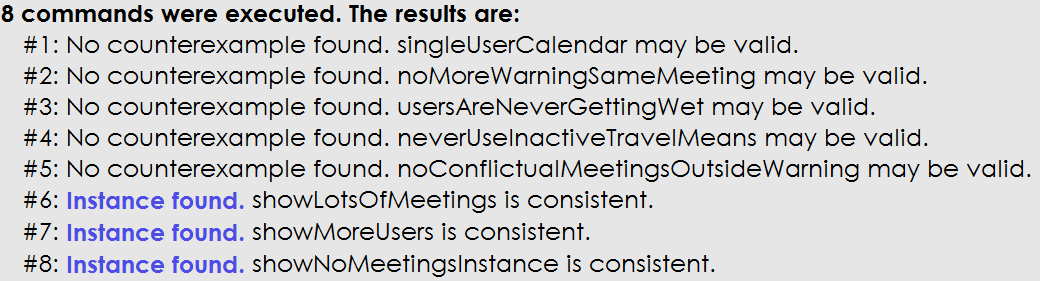
\includegraphics[width=\textwidth]{alloy/material/alloyresults} 
\caption{The results of the alloy model} 
\label{fig:alloyresults} 
\end{figure} 
\end{center}
\clearpage
\subsection{Worlds Generated}

\subsubsection{World One}

In extracting this World we decided to concentrate on a single user reality, in order to make it simpler to understand the usage of the application within the User context.
\\As you can easily see, what this diagram shows is the \textbf{Meeting} entity and the relationships it has with the \textbf{Travels}, the \textbf{Warnings} and the \textbf{Locations}.
\\Having a lot of meetings for a single user allows us to raise the probabilities to have conflicts between meetings, this is mainly because conflicts have to be in the same calendar (thus they have to be of the same User).
\\You can notice there are two Warnings, only connecting meetings with the \textbf{WithWarning status}, all meetings belonging to the warning are related to the each other and are connected to the warning, you can also see that there cannot exist two meetings in conflict with each other of which the appointment location is the same (obviously because if the user is already at the appointment site he cannot be late for the next meeting.
\\Another things to notice is that a meeting scheduled in a time where the weather forecast says it's going to rain, (\textbf{weather : Rainy}, where rainy symbolizes any type of 'bad weather') cannot have a \textbf{route} which involves the usage of means of transport where the user could wet himself (Bike, SharedBike, OnFoot).

\begin{figure} 

\begin{center}

\makebox[\textwidth]{%
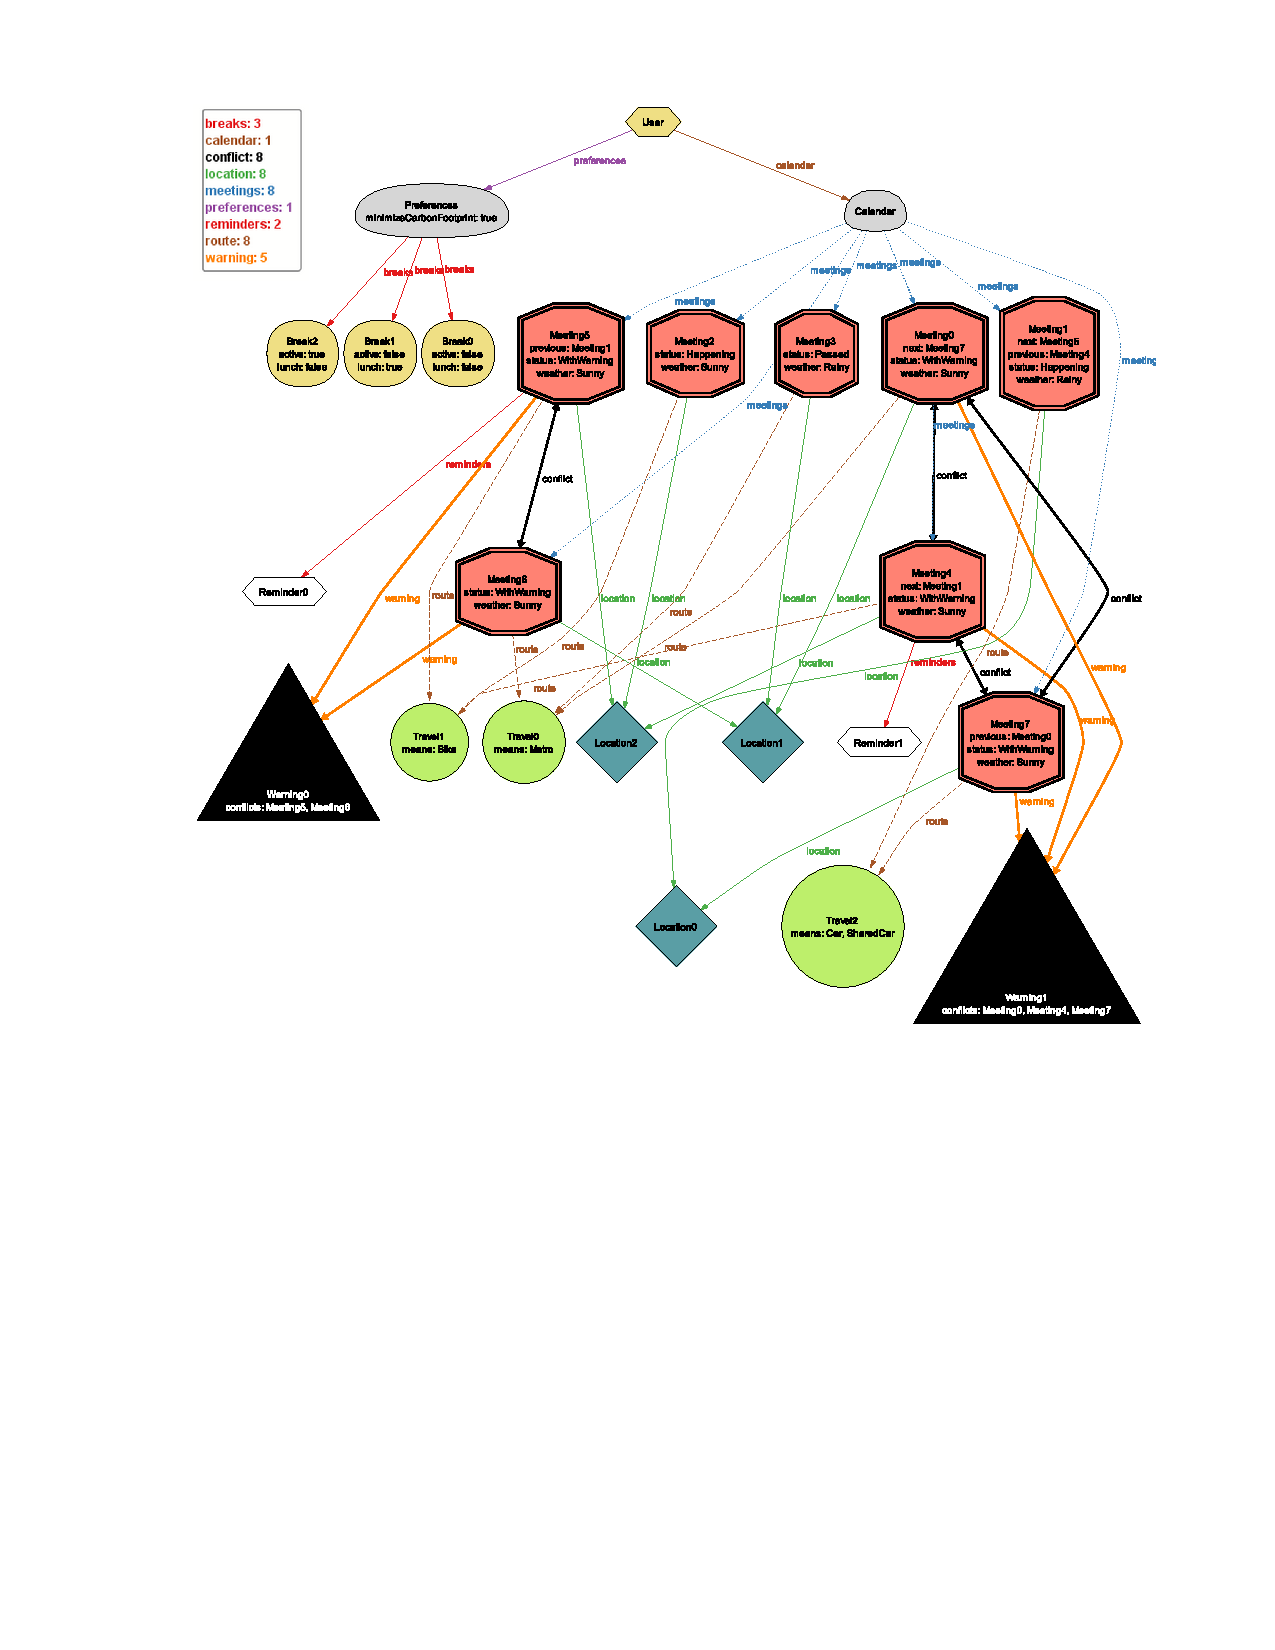
\includegraphics[width=1.7\linewidth]{alloy/world1pdf} 
}
\caption{Alloy World 1} 
\label{fig:alloyworld1} 


\end{center}
\end{figure} 

\clearpage
\subsubsection{World Two}

The second world was extracted in such a way that allow us to look for irregularities at the multi-client application, hence looking at consistency from the server-side.
\\We specified we wanted to have more than one User in order to be able to understand if the various meetings would not mix up neither between calendar nor between users.
\\An important thing that can be shown from this diagram is that the only warning is generated between two meetings belonging to the same Calendar (thus they are of the same User), and of course as we have seen in the previous world there cannot be meetings in conflict with each other if they are pointing at the same location.
\\The last thing to notice is that the Time relation symbolized by the previous relation and next relation works just fine, the next relation is the defined as the transposition of previous.


\begin{figure} 

\begin{center}

\makebox[\textwidth]{%
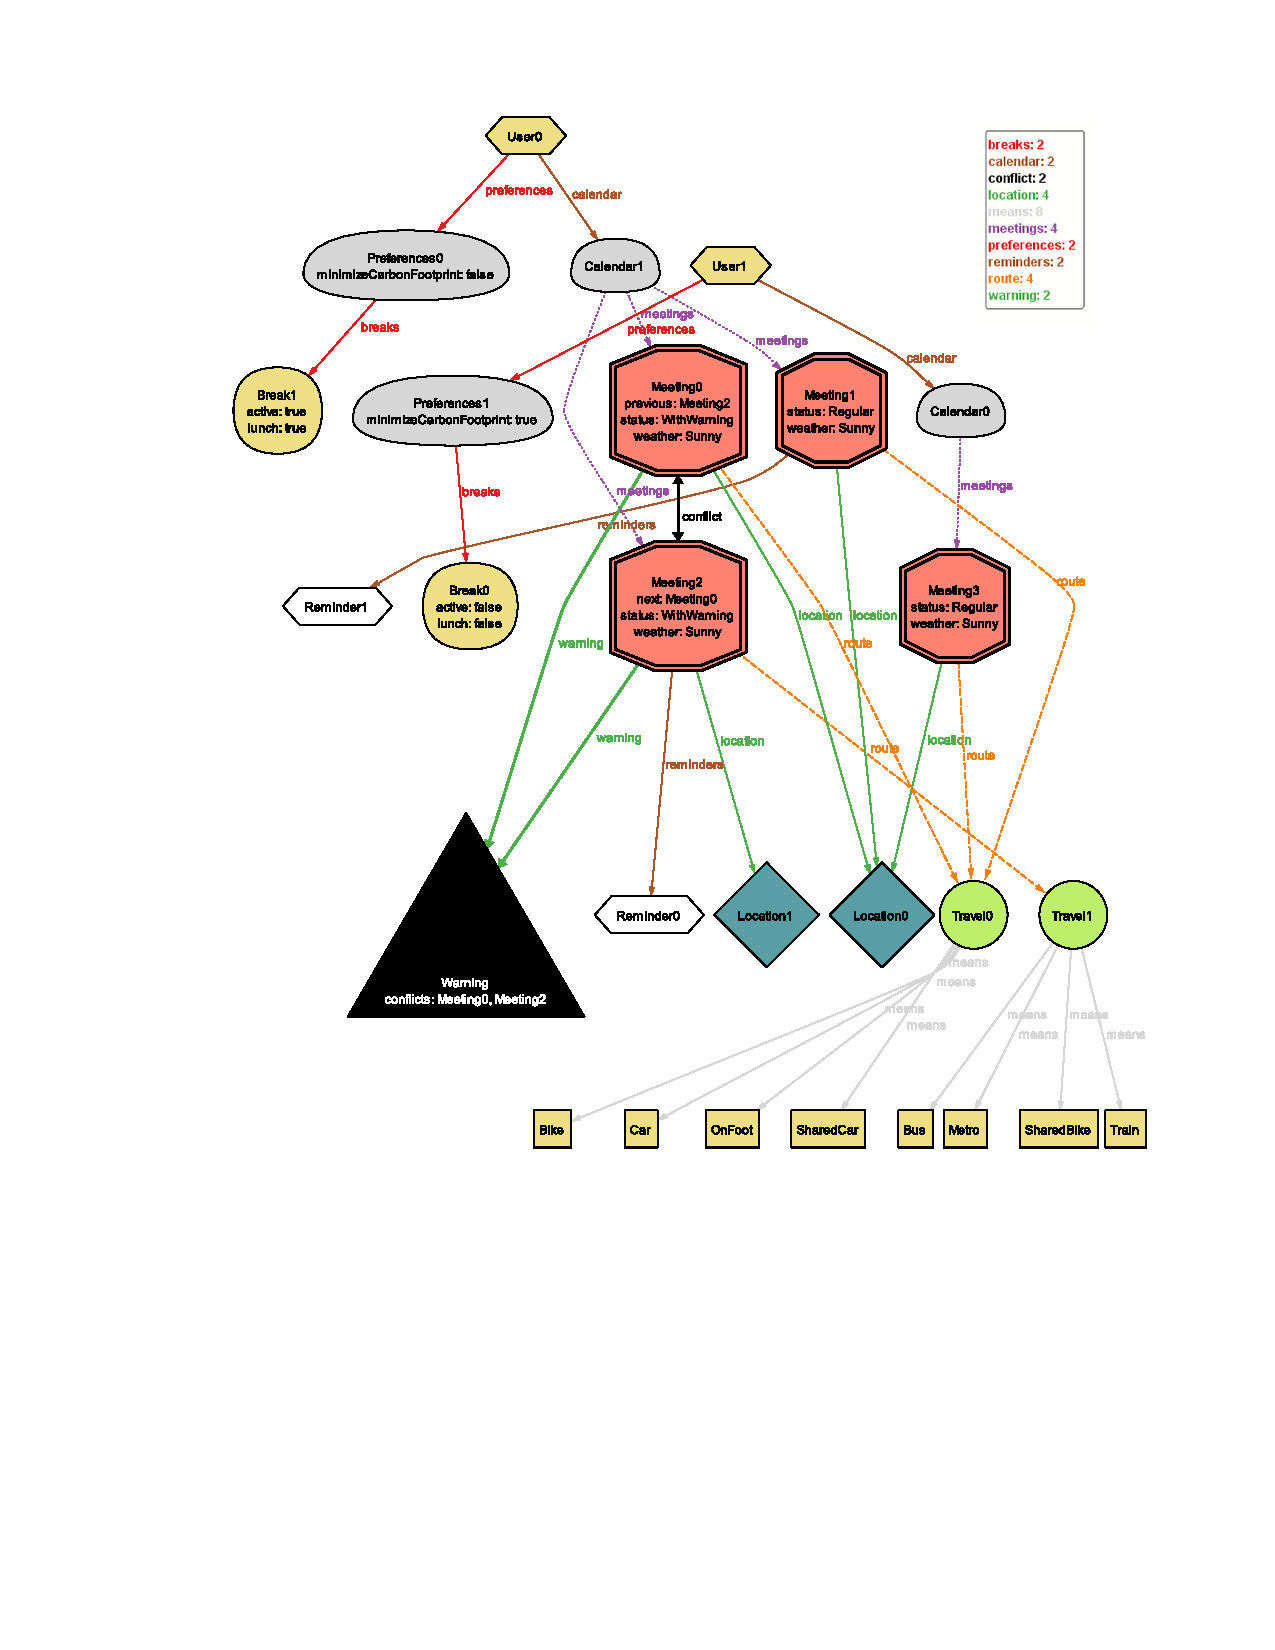
\includegraphics[width=1.6\linewidth]{alloy/world2pdf} 
}
\caption{Alloy World 2} 
\label{fig:alloyworld2} 


\end{center}
\end{figure} 


\clearpage
\section{Appendix}

\subsection{Used software}
\begin{center}
	
	\-\\
	\begin{tabular}{*{2}{c}}
		\toprule
		Task & Software \\
		\midrule
		Edit and compile \LaTeX\ code & TeXmaker, TeXstudio\\
		Development IDE & Netbeans\\
		Application server & Glassfish 4.1.1\\
		DBMS & Java DB (Derby)\\
		\bottomrule
	\end{tabular}
\end{center}

\subsection{Effort spent}

\end{document}
